% =============================================================================
% Working paper format (AEA style: Times, 1in margins, onehalfspacing body)
% =============================================================================
\documentclass[reqno,12pt]{article}
\usepackage[utf8]{inputenc}
\usepackage[margin=1in]{geometry}
\usepackage{mathptmx}
\usepackage[round, authoryear]{natbib}
\usepackage{amsmath, amssymb, dsfont, bbm, amsthm}
\usepackage{graphicx, booktabs, subcaption, float, placeins, multirow}
\usepackage{algorithm, algpseudocode}
\usepackage[table,dvipsnames]{xcolor}
\usepackage[bottom]{footmisc}
\usepackage[nodisplayskipstretch]{setspace}

\definecolor{paired10lightred}{RGB}{237, 159, 156}
\usepackage[colorlinks=true,
            linkcolor=NavyBlue,
            filecolor=blue,
            urlcolor=paired10lightred,
            citecolor=NavyBlue,
            pdftitle={Double Debiased Machine Learning for Difference-in-Differences under Imperfect Compliance},
            pdfauthor={Andres Mena}]{hyperref}

\DeclareMathOperator*{\argmax}{arg\,max}
\DeclareMathOperator*{\argmin}{arg\,min}

% Theorem environments
\theoremstyle{plain}
\newtheorem{assumption}{Assumption}
\newtheorem{proposition}{Proposition}
\newtheorem{theorem}{Theorem}
\newtheorem{corollary}{Corollary}
\newtheorem{conjecture}{Conjecture}
\newtheorem{lemma}{Lemma}

\theoremstyle{definition}
\newtheorem{remark}{Remark}

% Trimming assumptions (displayed as "Assumption T1", "Assumption T2", ...)
\newtheorem{tassumption}{Assumption}
\renewcommand{\thetassumption}{T\arabic{tassumption}}

% Proof sub-environments (upright body)
\newtheoremstyle{proofstyle}{6pt}{4pt}{\upshape}{}{\bfseries}{.}{0.5em}{}
\theoremstyle{proofstyle}
\newtheorem{propproof}{Proposition}
\newtheorem{theoremproof}{Theorem}

\newcommand{\propositionref}[1]{Proposition~\ref{#1}}

\begin{document}
 
\title{Double Debiased Machine Learning for Difference-in-Differences under Imperfect Compliance\thanks{I thank Susanne Schennach, Peter Hull, Toru Kitagawa, and Jonathan Roth for helpful comments and conversations, as well as participants in the Brown Econometrics Coffee for valuable feedback. All remaining errors are my own.}}
\author{Andres Mena\\Brown University}
\date{March 2026}
\maketitle

\begin{abstract}
\noindent This paper develops debiased machine learning estimators for difference-in-differences designs with imperfect compliance. I derive closed-form orthogonal scores for the Wald-DID and time-corrected estimands of \citet{fuzzy2018} and construct cross-fitted GMM estimators that are $\sqrt{n}$-consistent and asymptotically normal under standard rate conditions on the nuisance functions. I also propose a data-driven trimming rule that targets a sample analog of the estimator's asymptotic variance, excludes only observations whose probability of belonging to the treated group is close to one, and does not require knowledge of the treatment effect. Simulations suggest that the estimators achieve nominal coverage at moderate sample sizes. An application to the INPRES school construction program illustrates the method.
\end{abstract}

\medskip
\noindent\textbf{Keywords:} Difference-in-Differences, Machine Learning, Double Debiasing, Fuzzy DID, Propensity Score Trimming\\
\noindent\textbf{JEL:} C13, C14, C21, C55.

\newpage
\onehalfspacing

% --- Main body ---
\section{Introduction}

Difference-in-differences (DID) is among the most widely used methods for causal inference in non-experimental settings. In many applications, however, compliance is imperfect. Some units in the treated group do not take up treatment, and some in the control group do \citep[e.g.,][]{duflo2001schooling, cornelissen2018benefits, kennedy2023hidden}. In such \textit{fuzzy} designs, the standard DID estimand recovers only an intention-to-treat effect, which is known to understate the effects among the treated. \cite{fuzzy2018} show that the Wald-DID ratio, i.e.\ the DID in outcomes divided by the DID in treatment take-up, identifies a local average treatment effect (LATE) under monotonicity and treatment-effect stability, and propose a Time-Corrected (TC) variant that relaxes stability by using within-status outcome trends in the control group.

In order to relax identification assumptions, both Wald-DID and TC estimands can be extended to accommodate covariates. In modern applications the relevant covariate set can be high-dimensional, with the number of covariates potentially much larger than the sample size. Machine learning methods handle high dimensions through regularization, but the resulting first-step bias introduced by this type of learner contaminates plug-in treatment-effect estimators \citep{DDML2018}.

This paper develops debiased machine learning (DML) estimators for the Wald-DID and Time-Corrected estimands. I recast both estimands as unconditional moment restrictions and derive orthogonal scores for each using the first-step influence function approach of \citet{ichimura2022influence}. The resulting scores are locally robust in the sense of \citet{chernozhukov2022locally} and satisfy Neyman orthogonality. The cross-fitted GMM estimators built from them are $\sqrt{n}$-consistent and asymptotically normal under the standard $n^{-1/4}$ product-rate condition on the first-step nuisance estimates (Theorem~\ref{thm:1}). The orthogonal scores are proportional to the efficient influence functions of the two estimands, so the cross-fitted GMM estimators attain the semiparametric efficiency bound (Proposition~\ref{prop:4}). The framework accommodates flexible first-step learners, including Lasso, random forests, and neural networks.

\begin{figure}[H]
    \centering
    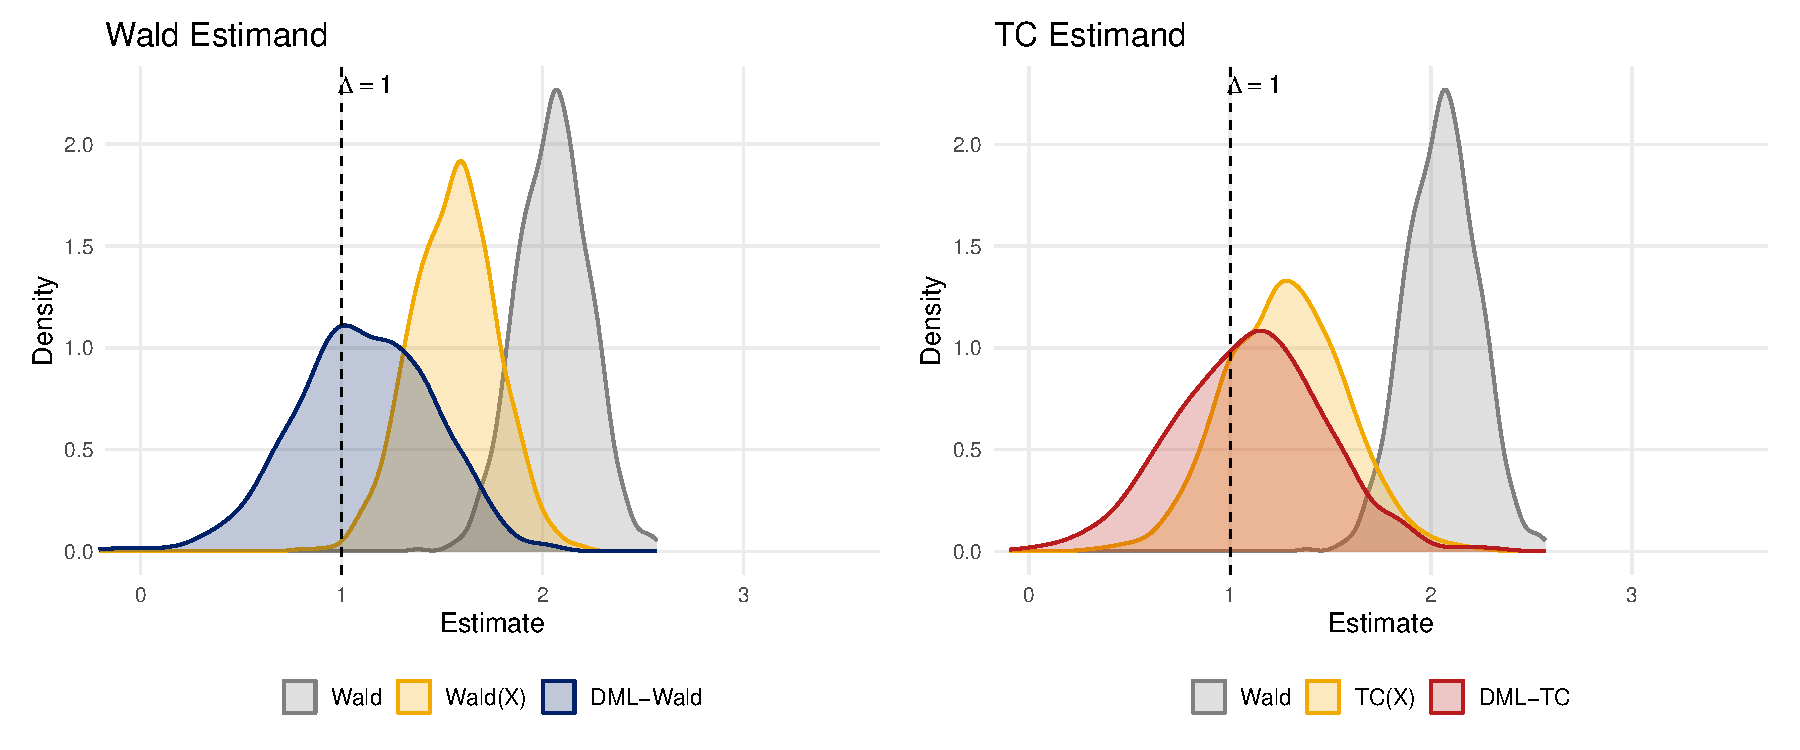
\includegraphics[width=\linewidth]{../output/figures/fig1_production.pdf}
    \caption[Sampling distribution of estimators]{Sampling distribution of estimators (true $\Delta=1$, dashed line; $n=5{,}000$, $p=100$ with 20 signal $+$ 80 noise, $M=1{,}000$). Left: Wald estimand. Right: TC estimand. The Wald estimator without covariates (grey, baseline in both panels) is consistent but noisy. The Lasso plug-in estimators (Wald$_X$, TC$_X$; gold) exhibit bias equal to 56\% and 28\% of the true effect. The DML estimators (DML-Wald in blue, DML-TC in red) reduce bias to 11\% and 10\%, attain 90--95\% coverage, and are centered near the truth.}\label{fig:1}
\end{figure}

A second contribution is a data-driven trimming algorithm for the propensity score. The proposed DML scores involve inverse-probability weights that become unstable when the probability of belonging to the treated group approaches one. Extending \cite{crump2009trimming} from the average treatment effect to our DID-IV estimands, I propose a data-driven, one-sided trimming rule that targets a sample analog of the estimator's asymptotic variance. The rule excludes only observations with high treatment probability, imposes no lower bound, and does not require knowledge of the true treatment effect. Monte Carlo simulations show it reduces variance and RMSE relative to fixed symmetric thresholds, at the cost of some bias because the trimmed estimand is not exactly the LATE. Appendix~\ref{sec:app_trimming} states formal optimality as a conjecture and derives the one-sided form under homoskedasticity and a weak monotonicity condition on the conditional first stage.

Monte Carlo simulations with $M=1{,}000$ replications confirm that DML-Wald and DML-TC attain near-nominal coverage at moderate sample sizes (Figure~\ref{fig:1}), while Lasso plug-in alternatives undercover by 17 to 46 percentage points. An application to the INPRES school construction program in Indonesia \citep{duflo2001schooling} uses a $p = 45$ individual-level dictionary and illustrates both contributions. Relative to the Lasso plug-in, the DML correction shifts point estimates downward across specifications and tightens cluster-robust confidence intervals at the primary-completion margin, and the trimming algorithm certifies common support when the propensity distribution stays interior.

The rest of the paper is organized as follows. Section~\ref{sec:lit} reviews the related literature. Section~\ref{sec:2} describes the Wald-DID and TC estimands. Section~\ref{sec:3} develops the locally robust estimators and states Theorem~\ref{thm:1}. Section~\ref{sec:4} presents the propensity score trimming algorithm. Section~\ref{sec:5} presents Monte Carlo evidence. Section~\ref{sec:6} applies the estimators to INPRES. Section~\ref{sec:7} concludes.

\section{Related Literature}\label{sec:lit}

This paper extends the fuzzy DID estimands of \cite{fuzzy2018} by deriving closed-form first-step influence functions for the Wald-DID and time-corrected estimands. The result is a debiased machine-learning formulation with analytic Riesz representers and a data-driven one-sided trimming rule. The contribution sits at the junction of three literatures: debiased ML for sharp DID, IV combined with DID, and influence-function tools for semiparametric efficiency.

In sharp DID, \cite{sant2020doubly} derive the semiparametric efficiency bound for the ATT and propose doubly robust estimators. \cite{chang2020double} bring this score into the DML framework for two-period DID with high-dimensional covariates, and \cite{callaway2023ddml} extend the same logic to staggered adoption with group-time parameters, building on \cite{callaway2021did}. More recent work sharpens efficiency and conditional identification: \cite{chen2025efficient} derive efficient event-study estimators, and \cite{caetano2024did} formalize DID identification under conditional parallel trends. All of these papers study sharp designs, where treatment status coincides with the group-time interaction.

A separate strand combines IV with DID under an external instrument. \cite{ye2023instrumented} develop instrumented DID and propose multiply robust semiparametric estimators for the ATE and CATE, \cite{zhao2025semiparametric} extend the framework to optimal policy learning, and \cite{miyaji2024instrumented} study heterogeneous effects and staggered instrument adoption. These papers do not use debiased machine learning or cross-fitting for high-dimensional covariates. The fuzzy DID design of \cite{fuzzy2018} is different: no external instrument is available, group-time variation itself supplies the instrument, and the target is a LATE for treatment-group switchers rather than an ATE.

Adapting debiased machine learning to the fuzzy design requires a first-step influence function that corrects for ML-estimated nuisances inside a ratio of moments. \cite{hahn1998} provides the classical semiparametric-efficiency benchmark for ATE-type problems, while \cite{newey1994asymptotic} and \cite{ichimura2022influence} give the pathwise-derivative tools behind the FSIF construction. \cite{chernozhukov2022locally} place these ideas in a locally robust GMM framework with cross-fitting, and \cite{CNS2022} and \cite{escanciano2023automatic} estimate Riesz representers numerically through penalized dictionary regressions. This paper instead derives the representers analytically. In the fuzzy DID setting they reduce to propensity-weighted cell indicators, which makes the sign structure transparent and avoids an auxiliary tuning step.

\section{Setup and Identification}\label{sec:2}

Let $W_i = (Y_i, D_i, G_i, T_i, X_i)$, $i = 1,\ldots,n$, be i.i.d.\ observations from a repeated cross-section. The outcome is $Y$, the binary treatment is $D$, the group assignment is $G \in \{0,1\}$, the time period is $T \in \{0,1\}$, and $X$ is a possibly high-dimensional vector of covariates. Potential outcomes are $Y(1)$ and $Y(0)$, with $Y = DY(1) + (1-D)Y(0)$. The design is \emph{fuzzy} because $D \neq GT$. Some treatment-group units remain untreated, and some control-group units take the treatment. Let $S = \{D_0 < D_1, G=1\}$ denote the \emph{switchers}, treatment-group units who are untreated at $T=0$ and treated at $T=1$. The parameter of interest is the LATE for these switchers,
\[
    \Delta = E[Y(1) - Y(0) \mid G=1, T=1, S=1].
\]

I follow the identification framework of \citet{fuzzy2018} and begin with the general assumptions shared by both estimands. Assumptions~\ref{ass:1}--\ref{ass:3} in Appendix~\ref{sec:app_setup} define the fuzzy DID environment. Assumption~\ref{ass:1} (Conditional Fuzzy Design) requires treatment take-up to rise more in the treatment group than in the control group. Assumption~\ref{ass:2} (Stable conditional percentage of treated units in the control group) keeps the control-group treatment share fixed over time within $X$ cells. Assumption~\ref{ass:3} (Treatment participation equation) is a monotonicity-type restriction indicating that conditional on $X$, units can switch treatment in only one direction within each group. Appendix~\ref{sec:app_setup} also reproduces the additional covariate assumptions used in the supplement's identification results.


\subsection{Estimands}\label{sec:2b}

For any random variable $R$, let $m^R_{gt}(x) = E[R \mid G=g, T=t, X=x]$ and $DID_R(X) = R - m^R_{10}(X) - m^R_{01}(X) + m^R_{00}(X)$.

Assumptions~\ref{ass:1}--\ref{ass:3} define the fuzzy DID environment. The Wald ratio identifies the treatment-group switcher LATE $\Delta$ once we add three conditions. Assumption~\ref{ass:4} imposes conditional common trends in untreated potential outcomes across the treatment and control groups. Assumption~\ref{ass:5} requires treatment effects to be stable over time within cells defined by baseline treatment status. The third point of Assumption~\ref{ass:8x} requires common covariate support across cells, so these conditional comparisons can be aggregated to recover $\Delta$. Under these conditions,
\begin{equation}\label{eq:Wdid}
    W^{DID} \equiv \frac{E[DID_Y(X)\mid G=1, T=1]}{E[DID_D(X)\mid G=1, T=1]} = \Delta.
\end{equation}
The numerator is the covariate-adjusted DID in outcomes, and the denominator is the corresponding DID in treatment take-up, both evaluated in the treated-post cell.

For the time-corrected estimand, let $\delta_d(X) = E[Y \mid D=d, G=0, T=1, X] - E[Y \mid D=d, G=0, T=0, X]$ denote the control-group time trend in $Y$ within baseline treatment-status cell $d$.

The time-corrected estimand replaces Assumptions~\ref{ass:4}--\ref{ass:5} with Assumption~\ref{ass:4prime}, which imposes conditional common trends within baseline treatment-status cells. Together with Assumptions~\ref{ass:1}--\ref{ass:3} and the third point of Assumption~\ref{ass:8x}, it identifies the same treatment-group switcher LATE $\Delta$:
\begin{equation}\label{eq:Wtc}
    W^{TC} \equiv \frac{E[Y - m^Y_{10}(X) - m^D_{10}(X)\delta_1(X) - (1-m^D_{10}(X))\delta_0(X)\mid G=1, T=1]}{E[D - m^D_{10}(X)\mid G=1, T=1]} = \Delta.
\end{equation}
The TC numerator subtracts a counterfactual outcome that combines two control-group time trends: $\delta_1(X)$ for units with baseline treatment status $D(0)=1$ and $\delta_0(X)$ for units with $D(0)=0$, weighted by the baseline treated share $m^D_{10}(X)$. The denominator is the corresponding adjusted change in treatment take-up.

\subsection{Plug-in Estimators}\label{sec:2c}

Given first-step estimates $\hat{m}^R_{gt}$ and $\hat{\delta}_d$, the plug-in estimators $\widehat{Wald}_X$ and $\widehat{TC}_X$ replace each unknown conditional expectation with its estimated counterpart:
\begin{equation*}
    \widehat{Wald}_X = \frac{\frac{1}{n_{11}} \sum_{i \in I_{11}}[Y_i - \hat{m}^Y_{10}(X_i) - \hat{m}^Y_{01}(X_i) + \hat{m}^Y_{00}(X_i)]}{\frac{1}{n_{11}} \sum_{i \in I_{11}}[D_i - \hat{m}^D_{10}(X_i) - \hat{m}^D_{01}(X_i) + \hat{m}^D_{00}(X_i)]}
\end{equation*}
\begin{equation*}
    \widehat{TC}_X = \frac{\frac{1}{n_{11}} \sum_{i \in I_{11}}[Y_i - \hat{m}^Y_{10}(X_i) - \hat{m}^D_{10}(X_i)\hat{\delta}_1(X_i) - (1-\hat{m}^D_{10}(X_i))\hat{\delta}_0(X_i)]}{\frac{1}{n_{11}} \sum_{i \in I_{11}}[D_i - \hat{m}^D_{10}(X_i)]}
\end{equation*}
where $I_{11}=\{i: G_i=1, T_i=1\}$ and $n_{11}=|I_{11}|$.

These estimators are consistent when $\hat\gamma$ converges to the true conditional means. But when $\hat\gamma$ comes from a regularized or model-selected first step, the plug-in estimators inherit first-step bias. Section~\ref{sec:3} constructs orthogonal scores that remove this bias and restore valid inference.

\section{Locally Robust Estimators}\label{sec:3}

This section develops locally robust scores for the Wald-DID and time-corrected Wald estimands. I rewrite each target parameter as an unconditional moment restriction, $E[g(W,\gamma,\theta)]=0$, and use the first-step influence function approach of \citet{ichimura2022influence} within the locally robust framework of \citet{chernozhukov2022locally} to construct orthogonal scores. Each identifying moment is augmented with a correction term that removes the first-order effect of estimating the nuisance vector $\gamma$. The FSIF construction yields an orthogonal score whose correction term is a linear combination of first-step prediction errors:
\[
\psi(W,\gamma,\alpha,\theta)=g(W,\gamma,\theta)+\alpha(W)^\top\bigl(R-\gamma(X)\bigr),
\]
where $R$ collects the random variables whose conditional expectations define the nuisance components and $\alpha$ is the vector of Riesz representers. The derivations below show that the derived Riesz representers $\alpha$, when evaluated at their true value $\alpha_0$, satisfy the Neyman orthogonality condition of \citet{DDML2018}:
\[
\partial_\gamma E[\psi(W,\gamma,\alpha_0,\theta_0)]\big|_{\gamma=\gamma_0}=0.
\]
so first-step estimation errors affect the moment condition only through higher-order terms. The orthogonal scores derived below are proportional to the efficient influence functions in \citet{fuzzy2018}, so after normalization they imply the same semiparametric efficiency bound. I use the FSIF route because it delivers the explicit decomposition $\psi = g + \phi$ and the closed-form Riesz representers needed for cross-fitted GMM estimation and for the trimming analysis in Section~\ref{sec:4}.


\subsection{Identifying Moment Functions}\label{sec:3a}

I first restate the Wald-DID and time-corrected estimands in Equations~\eqref{eq:Wdid} and~\eqref{eq:Wtc} as unconditional moment restrictions. The purpose is to define a population moment functional with a clear zero at the target parameter. The ratios in Equations~\eqref{eq:Wdid} and~\eqref{eq:Wtc} identify $\Delta$ inside the treated-post cell, $(G,T)=(1,1)$. Moving the numerator to the left-hand side and averaging with the weight $GT/p_{11}$, where $p_{11}=\Pr(G=1,T=1)$, gives equivalent restrictions that equal zero at the true parameter. For the Wald-DID estimand,

\begin{equation}\label{eq:3}
    E\left[\frac{GT}{p_{11}}(DID_Y(X)-DID_D(X)\Delta)\right]=0
\end{equation}
For the TC estimand,
 \begin{equation}\label{eq:4}
    E\Bigl[\frac{GT}{p_{11}}\bigl(Y-m^Y_{10}(X)-m^D_{10}(X)\delta_1(X)-(1-m^D_{10}(X))\delta_0(X)-(D-m^D_{10}(X))\Delta\bigr)\Bigr]=0
 \end{equation}

This step is algebraic. It does not change the estimand or add an identifying assumption. It turns each conditional ratio into a population object that can be differentiated with respect to the first-step nuisance functions. The pointwise moment functions are
\begin{equation}
        \begin{aligned}\label{eq:5}
            g^{wald}(W,\gamma^{wald},\theta) &= \frac{GT}{p_{11}}[(Y-m^Y_{10}(X)-m^Y_{01}(X)+m^Y_{00}(X)) \\
                                                             &\quad - (D-m^D_{10}(X)-m^D_{01}(X)+m^D_{00}(X))\theta]
        \end{aligned}
    \end{equation}



    \begin{equation}\label{eq:6}
        \begin{aligned}
            g^{tc}(W,\gamma^{tc},\theta) &= \frac{GT}{p_{11}}[(Y-m^Y_{10}(X)-\delta_1(X)m^D_{10}(X)-(1-m^D_{10}(X))\delta_0(X)) \\
                                                             &\quad - (D-m^D_{10}(X))\theta]
        \end{aligned}
    \end{equation}
where $\mu^Y_{dgt}(x)=E[Y \mid D=d, G=g, T=t, X=x]$ and $\delta_d(X)=\mu^Y_{d01}(X)-\mu^Y_{d00}(X)$. The nuisance vectors are $\gamma^{wald} = \{m^Y_{gt}, m^D_{gt}\}_{(g,t) \neq (1,1)}$ and $\gamma^{tc} = \{m^Y_{10}, m^D_{10}, \mu^Y_{d0t}\}_{d,t \in \{0,1\}}$.

These pointwise moments induce the population functionals
\[
    \mathcal{M}^j(\gamma^j,\theta)
    =
    E\bigl[g^j(W,\gamma^j,\theta)\bigr],
    \qquad j\in\{\text{wald},\text{tc}\}.
\]
At the true nuisance vector $\gamma^j_0=\gamma^j(F_0)$, the target parameter solves $\mathcal{M}^j(\gamma^j_0,\Delta)=0$. This functional is the object differentiated in Section~\ref{sec:3b}. Once it is explicit, the first-step influence function follows from the directional derivative of $\mathcal{M}^j$ in the directions of the nuisance functions estimated in the first step.

\begin{proposition}\label{prop:1}
At the true nuisance vectors, the pointwise moments in \eqref{eq:5} and \eqref{eq:6} generate the same zero restrictions as the centered estimands in \eqref{eq:Wdid} and \eqref{eq:Wtc}:
\[
    E[g^{wald}(W,\gamma^{wald}_0,\theta)]=0
    \quad\Longleftrightarrow\quad
    W^{DID}-\theta=0,
\]
and
\[
    E[g^{tc}(W,\gamma^{tc}_0,\theta)]=0
    \quad\Longleftrightarrow\quad
    W^{TC}-\theta=0.
\]
Therefore, under the corresponding identification assumptions, both moment functions identify the same target $\Delta$.
\end{proposition}


Proposition~\ref{prop:1} makes the population target for plug-in GMM explicit. Solving $E[g^j(W,\gamma^j_0,\theta)]=0$ is equivalent to solving $W^{DID}-\theta=0$ for the Wald-DID moment and $W^{TC}-\theta=0$ for the TC moment, so if the first-step estimates converge to $\gamma^j_0$, the sample analog of $\mathcal{M}^j(\hat\gamma^j,\theta)=0$ targets the same $\Delta$. But this population statement does not describe the leading error from estimating $\gamma^j$. The next remark isolates that error and shows the term the FSIF must cancel.

\begin{remark}[Exact first-order bias of plug-in estimators]\label{cor:bias}
Let $\hat\theta_{\text{plug-in}}$ denote the estimator that replaces the unknown nuisance functions in $g^j$ with first-step estimates $\hat\gamma^j$ and then solves the resulting sample moment condition. A first-order expansion around $(\gamma^j_0,\Delta)$ gives
\begin{equation}\label{eq:plugin_bias_linearization}
    \hat\theta_{\text{plug-in}} - \Delta
    =
    -\frac{1}{G^j}\frac{1}{n}\sum_{i=1}^n g^j(W_i,\gamma^j_0,\Delta)
    -
    \underbrace{\frac{\dot{\mathcal{M}}^j_{\gamma^j_0}[\hat\gamma^j-\gamma^j_0]}{G^j}}_{\text{first-order bias}}
    + o_P(n^{-1/2}),
\end{equation}
where $G^j = \partial_\theta E[g^j(W,\gamma^j,\theta)]|_{\theta=\Delta}$ and $\dot{\mathcal{M}}^j_{\gamma^j_0}[h]$ is the Gateaux derivative of $\mathcal{M}^j(\gamma^j,\Delta)$ with respect to $\gamma^j$, evaluated at $\gamma^j_0$ in direction $h$. The second term is the leading bias from first-step estimation. It is the directional derivative of the identifying functional in the direction of the estimation error $\hat\gamma^j-\gamma^j_0$. Section~\ref{sec:3b} uses this derivative to construct the correction term $\phi^j$ that cancels the first-order channel at $\gamma^j_0$.
\end{remark}


\subsection{The First Step Influence Function}\label{sec:3b}

Remark~\ref{cor:bias} shows why the plug-in approach falls short. Even when consistent, the leading error contains a first-order term from estimating $\gamma$, and with regularized first steps that term need not be small relative to the $n^{-1/2}$ sampling noise. The first-step influence function (FSIF) of \citet{ichimura2022influence} and \citet{chernozhukov2022locally} is designed to remove that term. I derive it by computing the Gateaux derivative of $E[g^j(W,\gamma^j(F_\tau),\theta)]$ along smooth contamination paths $F_\tau = (1-\tau)F_0 + \tau H$ and reading off the function $\phi^j$ that satisfies $\partial_\tau E[g^j]\big|_{\tau=0} = E[\phi^j]$. Because $g^j$ is linear in each component of $\gamma$, this Gateaux derivative reduces to a sum of $K_j$ component-wise corrections. The FSIF is
\begin{equation}\label{eq:fsif_decomp}
    \phi^{j}(W,\gamma^j,\alpha^j,\theta)
    \;=\;
    \sum_{k=1}^{K_j}
    \underbrace{\alpha^{j}_k(W)}_{\text{Riesz representer}}\,
    \underbrace{\bigl(R^{j}_k-\gamma^{j}_k(X)\bigr)}_{\text{prediction error}}.
\end{equation}
Each term multiplies a first-step prediction error by a weight that records how perturbations of that nuisance function shift the identifying moment. Together, these terms reconstruct the first-order error from Remark~\ref{cor:bias}.

\paragraph{FSIF example} Consider one component of the Wald nuisance vector $\gamma^{wald} = \{m^Y_{gt}, m^D_{gt}\}_{(g,t)\neq(1,1)}$, namely $m^Y_{10}(X) = E[Y \mid G=1,T=0,X]$, the treated-group pre-period outcome regression. The object differentiated is the population moment $E[g^{wald}(W,\gamma^{wald},\theta)]$, viewed as a functional of $\gamma^{wald}$. Taking its Gateaux derivative with respect to a perturbation in the $m^Y_{10}$ component of $\gamma^{wald}$ produces the FSIF term, expressed in terms of the cell propensity $\pi_{gt}(X) = \Pr(G=g, T=t \mid X)$,
\begin{equation}\label{eq:fsif_example}
    \phi^{wald}_{m^Y_{10}}(W)
    \;\equiv\; \alpha^{wald}_{m^Y_{10}}(W)\cdot\bigl(Y - m^Y_{10}(X)\bigr)
    \;=\; -\underbrace{\frac{\mathbf{1}\{G=1,T=0\}\,\pi_{11}(X)}{\pi_{10}(X)\,p_{11}}}_{\alpha^{wald}_{m^Y_{10}}(W)\,:\;\text{Riesz representer}}
    \,\cdot\,\underbrace{\bigl(Y - m^Y_{10}(X)\bigr)}_{\text{prediction error}}.
\end{equation}
This $\phi^{wald}_{m^Y_{10}}(W)$ is the $k$th term in the sum~\eqref{eq:fsif_decomp}, the one associated with $\gamma^{wald}_k = m^Y_{10}$. The indicator picks out observations actually in the $(G=1, T=0)$ cell, so only treated-group pre-period units contribute. The denominator $\pi_{10}(X) = \Pr(G=1, T=0 \mid X)$ is the conditional probability of being in that cell, and the ratio $\pi_{11}(X)/\pi_{10}(X)$ reweights those units so they speak to the target cell $(G=1, T=1)$. The remaining five Wald representers and the six TC representers follow the same template with their own cell indicators and propensity ratios. Appendix~\ref{sec:app_fsif} contains the full Gateaux-derivative computation, the closed forms of all $\alpha^j_k$, and the element-by-element expressions for $\phi^{wald}$ and $\phi^{tc}$.

\begin{proposition}[Closed-form first-step influence functions]\label{prop:2}
For $j\in\{\text{wald},\text{tc}\}$, let
\[
    \mathcal{M}^j(\gamma^j,\theta)
    =
    E\bigl[g^j(W,\gamma^j,\theta)\bigr]
\]
denote the population moment functional. The first-step influence function of $\mathcal{M}^j$ with respect to the nuisance vector $\gamma^j$ is
\[
    \phi^{j}(W,\gamma^j,\alpha^j,\theta)
    =
    \sum_{k=1}^{K_j}
    \alpha^{j}_k(W)\bigl(R^{j}_k-\gamma^{j}_k(X)\bigr),
\]
where $R^j_k$ is the random variable whose conditional expectation defines $\gamma^j_k$, and $K_j$ indexes the component-wise corrections for score $j$. The closed-form Riesz representers $\alpha^j_k$ are given in Appendix~\ref{sec:app_fsif}, Equations~\eqref{eq:fsif_wald_alpha_app}--\eqref{eq:fsif_tc_alpha2_app}; the resulting element-by-element expressions for $\phi^{wald}$ and $\phi^{tc}$ are Equations~\eqref{eq:8_app}--\eqref{eq:9_app}.
\end{proposition}

Proposition~\ref{prop:2} gives the core objects used in the rest of the theory. The Riesz representers $\alpha^j_k$ are the weights that translate a perturbation in each first-step nuisance function into its effect on the population moment. The FSIFs $\phi^{wald}$ and $\phi^{tc}$ then collect these weighted prediction errors into the correction added to $g^j$. These objects make it possible to form the locally robust score, implement the cross-fitted estimators, and study the variance effects of the cell weights. I derive the closed forms in Appendix~\ref{sec:app_fsif}, which lists all Wald and TC representers and the element-by-element formulas for $\phi^{wald}$ and $\phi^{tc}$.

\paragraph{Additional nuisance functions.} The FSIF correction is not free. The original moment $g^j$ requires only the conditional means in $\gamma^j$. The augmented score $\psi^j$ also requires additional cell propensities, $\pi_{gt}(X)$ for Wald-DID and $\pi_{dgt}(X)$ for TC, because they enter the Riesz representers in the denominator. These propensities must be estimated, typically by cross-fitted logit or random forest, so small estimated cell probabilities translate into large weights and high variance.

This variance problem is concentrated in the control-group cells. For treated-group cells, the relevant propensity ratio is constant in $X$. For control-group cells, the ratio is proportional to $e(X)/(1-e(X))$, where $e(X)=\Pr(G=1\mid X)$, so it grows large as $e(X)$ approaches one. TC tempers this problem by conditioning further on $D$, but it also requires more propensities to be estimated. Section~\ref{sec:4} addresses the resulting variance inflation with a trimming rule that removes observations with very high $\hat e(X)$ before averaging.


\subsection{Local Robustness and Orthogonality}\label{sec:3c}

Using the FSIF from Proposition~\ref{prop:2}, define the augmented score
\begin{equation}\label{eq:orth_score}
    \psi^{j}(W,\gamma^j,\alpha^j,\theta)
    \;=\;
    g^{j}(W,\gamma^j,\theta)
    +
    \phi^{j}(W,\gamma^j,\alpha^j,\theta).
\end{equation}
This subsection shows that the augmentation leaves the identifying restriction unchanged and removes the first-order sensitivity of the score to nuisance-estimation error. Proposition~\ref{prop:3} collects these two facts.

\paragraph{Mean-zero correction.} For $j \in \{\text{wald},\text{tc}\}$,
\begin{equation}\label{eq:fsif_meanzero}
    E\bigl[\phi^j(W,\gamma^j_0,\alpha^j,\theta)\bigr] = 0
    \quad \text{for every admissible $\alpha^j$ and every $\theta$.}
\end{equation}
Each Riesz representer contains a cell indicator, so observations outside the relevant cell drop out. Inside the cell, the residual is the prediction error from the nuisance regression that defines that component, so its conditional mean is zero by construction. Appendix~\ref{sec:app_proof_prop3} gives the formal computation.

Equation~\eqref{eq:fsif_meanzero} implies that the augmented score and the original identifying moment have the same expectation at the truth:
\begin{equation}\label{eq:psi_eq_g}
    E\bigl[\psi^j(W,\gamma^j_0,\alpha^j,\theta)\bigr]
    \;=\;
    E\bigl[g^j(W,\gamma^j_0,\theta)\bigr].
\end{equation}
So the FSIF correction does not change the target parameter and does not add new identifying restrictions. A GMM estimator built from $\psi^j$ still targets the same $\Delta$ as one built from $g^j$.

\paragraph{Neyman orthogonality.} The second property is that the Gateaux derivative of $E[\psi^j]$ with respect to $\gamma^j$ vanishes at $\gamma^j_0$:
\begin{equation}\label{eq:neyman_orth}
    \frac{\partial}{\partial \tau}
    E\bigl[\psi^j(W,\gamma^j_0 + \tau\delta,\alpha^j_0,\theta)\bigr]
    \bigg|_{\tau=0}
    \;=\; 0
\end{equation}
for every admissible direction $\delta$. Small perturbations of $\gamma^j$ around the truth therefore have no first-order effect on the expected score. This is exactly the first-order plug-in bias in Equation~\eqref{eq:plugin_bias_linearization}, and the FSIF correction is constructed to remove it. Appendix~\ref{sec:app_proof_prop3} provides the component-wise verification.

\begin{proposition}[Local robustness of $\psi^{wald}$ and $\psi^{tc}$]\label{prop:3}
For $j \in \{\text{wald},\text{tc}\}$ and any $\theta \in \Theta$, the augmented score $\psi^j = g^j + \phi^j$ satisfies
\begin{enumerate}
\item \textit{Mean-zero correction.} $E[\phi^j(W,\gamma^j_0,\alpha,\theta)] = 0$ for every admissible $\alpha$, so $E[\psi^j(W,\gamma^j_0,\alpha,\theta)] = E[g^j(W,\gamma^j_0,\theta)]$.
\item \textit{Neyman orthogonality.} $\partial_\tau\, E[\psi^j(W,\gamma^j_0 + \tau\delta,\alpha^j_0,\theta)]|_{\tau=0} = 0$ for every admissible direction $\delta$.
\end{enumerate}
See Appendix~\ref{sec:app_proof_prop3} for the component-wise proof.
\end{proposition}

Proposition~\ref{prop:3} has two claims. First, the correction term $\phi^j$ has mean zero when the nuisance vector $\gamma^j$ is evaluated at the truth. Therefore adding $\phi^j$ to $g^j$ does not change the identifying restriction. Second, the expected augmented score is flat, to first order, with respect to small perturbations of $\gamma^j$ around $\gamma^j_0$. Together, these cancellations are the local-robustness condition in \citet[Equation~4.1]{chernozhukov2022locally}. The FSIF decomposition of \citet[Equation~2.6]{ichimura2022influence} supplies the correction term $\phi^j$ that makes the cancellation possible.

\begin{remark}[Intuition for local robustness]\label{rmk:local_vs_double}
Local robustness means that the moment condition is protected against small first-step mistakes around the true nuisance functions. The plug-in moment $g^j(W,\hat\gamma^j,\theta)$ inherits the first-order error from estimating $\gamma^j$. The augmented score $\psi^j=g^j+\phi^j$ removes that first-order channel. The correction $\phi^j$ is built so that, at the truth, it averages to zero and offsets the first-order change in $E[g^j]$ caused by perturbing $\gamma^j$.

This is the sense in which the correction makes DDML stable. The estimator still uses estimated nuisance functions, but small errors in those first steps do not enter the final moment directly. They enter only through higher-order terms left after the first-order cancellation. Thus the role of $\phi^j$ is not to change the target parameter. Its role is to make the estimating equation less sensitive to the nuisance estimates used to construct it.
\end{remark}

\subsection{Locally Robust GMM Estimators}\label{sec:3d}
The locally robust score $\psi^j = g^j + \phi^j$ constructed in Section~\ref{sec:3c} can now be turned into a point estimator via cross-fitted GMM. To estimate the Local Average Treatment Effect (LATE) $\Delta$, I employ a Generalized Method of Moments (GMM) approach \citep{hansen1982large, newey1994large} that incorporates cross-fitting in the first step. This adjustment, inspired by \cite{DDML2018}, aims to relax the Donsker conditions and mitigate own-observation bias. Cross-fitting involves partitioning $\{1,\ldots,n\}$ into $L$ disjoint subsets $I_1,\ldots,I_L$ of size $n/L$. Then, I estimate functions $\hat{\gamma}_l$ and $\hat{\alpha}_l$ using observations outside fold $l$. Subsequently, I plug in estimated nuisance parameters into the identifying moment function $\hat{g}(W_i, \hat{\gamma}_l, \theta)$ and their respective influence function $\hat{\phi}(W_i, \hat{\gamma}_l, \hat{\alpha}_l, \theta)$  to construct a debiased sample moment function $\hat{\psi}(\theta)_{il}$ as follows:

\[
\hat{\psi}(\theta)_{il} = \hat{g}(W_i, \hat{\gamma}_l, \theta) + \hat{\phi}(W_i, \hat{\gamma}_l, \hat{\alpha}_l, \theta)
\]

The GMM estimator of the LATE is derived by minimizing the quadratic form of the sum of the debiased sample moment functions. Consequently, the proposed estimators, DML-Wald and DML-TC, are the sample analogs of the orthogonal moment condition $E[\psi^j(W, \gamma_0, \alpha_0, \theta_0)] = 0$, and are given by Equations~\ref{eq:13} and~\ref{eq:14}:


\begin{equation}\label{eq:13}
    \widehat{DML}^{wald} = \underset{\theta \in \Theta}{\text{argmin}} \; \bigg[\frac{1}{n}\sum^L_{l=1} \sum_{i\in I_l} \hat{\psi}^{wald}_{il}\bigg]^2
    \end{equation}

    \begin{equation}\label{eq:14}
    \widehat{DML}^{tc} = \underset{\theta \in \Theta}{\text{argmin}} \; \bigg[\frac{1}{n}\sum^L_{l=1} \sum_{i\in I_l} \hat{\psi}^{tc}_{il}\bigg]^2
    \end{equation}

Because the orthogonal scores are affine in $\theta$, the cross-fitted GMM criterion can be solved by the corresponding closed-form root once the nuisance functions are fixed.

Relative to naive plug-in estimators, DML-Wald and DML-TC learn nuisance functions on auxiliary folds and evaluate the score out of sample. The FSIF correction then removes the leading first-step bias, so the root is built from locally robust, cross-fitted moments rather than raw plug-in conditional means. The main practical issue is instability in the Riesz-weighted components when estimated cell propensities are small. Section~\ref{sec:4} addresses this with one-sided trimming.

\subsection{Asymptotic Properties}\label{sec:3e}

The main result of this section is Theorem~\ref{thm:1} which states that the $\widehat{DML}^{wald}$ and $\widehat{DML}^{tc}$ estimators achieve $\sqrt{n}$-consistency and asymptotic normality as long as the first-step estimators converge at rates faster than $n^{-1/4}$. Under standard regularity conditions on the nuisance parameters, this rate of convergence can be achieved by many machine learning methods including Lasso, logit-Lasso, random forests, and neural networks.

Let $\eta^{gt} = (m^Y_{gt}, m^D_{gt}, \pi_{gt})$ collect all nuisance functions for cell $(g,t)$. Let $\rho^R_{gt}=R-m^R_{gt}(x)$ be the residual of the nuisance function $m^R_{gt}(x)$ such that $E_{F}[\rho^R_{gt}|G=g, T=t, X]=0$, and $\eta^{gt}_0=(m^Y_{gt}(X),m^D_{gt}(X),\pi_{gt}(X))$ be the nuisance functions evaluated at $G=g,T=t$ and $F_0$. Let $c, C$ and $q$ be fixed strictly positive constants such that $q>2$. Consider also the sequences $\epsilon_n, P_n$ converging to $0$ such that $\epsilon_n = o(n^{-1/4})$, which implies $(\epsilon_n)^2 = o(n^{-1/2})$. Moreover, for any $\eta^{gt}=(l^{Y}_{gt}, l^{D}_{gt}, l^{\pi}_{{gt}})$ where $l^{Y}_{gt}$ is a function mapping from $(G,T,X)$ to $\mathbb{R}$ and $l^{D}_{gt}, l^{\pi}_{{gt}}$ are functions mapping from $(G,T,X)$ to $(\varepsilon, 1-\varepsilon)$ for some $\varepsilon \in (0,1/2)$ denote $\| \eta^{gt} \|_{F,q} = \max \{ \| l^Y_{gt} \|_{F,q}, \| l^D_{gt} \|_{F,q}, \| l^{\pi}_{gt} \|_{F,q} \}
$\\

\noindent
\textbf{Regularity Conditions.} {\itshape Let $F$ be any CDF of the random vector $W=(Y,D,G,T,X)$, then:
\begin{enumerate}
    \item[1.] (Bounded outcomes) \( \| Y \|_{F,q} \leq C \)
    \item[2.] (Overlap) \( \Pr_F(\varepsilon \leq e(X) \leq 1-\varepsilon) = 1 \), where $e(X) = \Pr(G=1 \mid X)$
    \item[3.] (Relevant first stage) \( |G^j| = |\partial_\theta E[g^j(W,\gamma^j,\theta)]\big|_{\theta=\Delta}| \geq c \)
    \item[4.] (Bounded conditional variance) \( \| E_F[(\rho^Y_{gt})^2|X] \|_{F,\infty} \leq C \)
    \item[5.] (First-step quality) Given a random subset \( I \) of \( [n] \) of size \( n_l = |I| \), the nuisance function estimator \( \hat{\eta}^{gt}(W_{i \in I}) \) obeys with probability at least \( 1-P_n \):
    \begin{enumerate}
        \item[(a)] (Bounded estimates) \( \| \hat{\eta}^{gt} - \eta^{gt} \|_{F,q} \leq C \)
        \item[(b)] (Consistency) \( \| \hat{\eta}^{gt} - \eta^{gt} \|_{F,2} \leq \epsilon_n \)
        \item[(c)] (Estimated overlap) \( \| \hat{\pi}^{gt} - 1/2 \|_{F,\infty} \leq 1/2 - \varepsilon \)
        \item[(d)] (Product rate) \( \| \hat{\pi}_{gt} - \pi_{gt} \|_{F,2} \cdot \| \hat{m}^{R}_{gt} - m^{R}_{gt} \|_{F,2} = o_P(n^{-1/2}) \) for $R\in\{Y,D\}$ and $(g,t)\neq(1,1)$
        \item[(d')] (TC product rate) \( \| \hat{\delta}_d - \delta_d \|_{F,2} \cdot \| \hat{m}^D_{10} - m^D_{10} \|_{F,2} = o_P(n^{-1/2}) \) for $d \in \{0,1\}$
    \end{enumerate}
\end{enumerate}

}
\medskip
Conditions 1--4 impose standard regularity on the outcome distribution, overlap, first-stage relevance, and conditional variances. The key requirement is Condition 5(d), the product rate. It asks that the propensity score estimation error and the conditional expectation estimation error, multiplied together, vanish faster than $n^{-1/2}$. A sufficient condition is that each first-step estimator converges faster than $n^{-1/4}$. Asymmetric rates also work. If the propensity score converges at rate $n^{-a}$ and the conditional expectation at rate $n^{-b}$, the requirement is $a + b > 1/2$. This is Condition 3.4(c) in \cite{DDML2018} and Assumption 3.1(f) in \cite{chang2020double}, and is achieved by Lasso under approximate sparsity and by random forests under smoothness assumptions.
\medskip

\begin{theorem}[$\sqrt{n}$-consistency and asymptotic normality]\label{thm:1}
Suppose Assumptions~\ref{ass:1}--\ref{ass:3} and Regularity Conditions 1--5 hold. Let $\widehat{DML}^{wald}$ and $\widehat{DML}^{tc}$ be the cross-fitted estimators defined in~\eqref{eq:13}--\eqref{eq:14} with $L$ folds.
\begin{enumerate}
    \item[\textup{(i)}] Under Assumptions~\ref{ass:4}--\ref{ass:5} and the third point of Assumption~\ref{ass:8x},
    $\;\sqrt{n}\,(\widehat{DML}^{wald}-\Delta) \xrightarrow{d} \mathcal{N}(0,\, V^{wald})$.
    \item[\textup{(ii)}] Under Assumption~\ref{ass:4prime} and the third point of Assumption~\ref{ass:8x},
    $\;\sqrt{n}\,(\widehat{DML}^{tc}-\Delta) \xrightarrow{d} \mathcal{N}(0,\, V^{tc})$.
\end{enumerate}
The asymptotic variance is $V^{j}=[G^{j}]^{-2}\,E[(\psi^{j})^2]$, where $G^{j}=\partial_\theta E[g^j(W, \gamma^j,\theta)]\big|_{\theta=\Delta}$ for $j\in\{\textup{wald}, \textup{tc}\}$.
\end{theorem}

\paragraph{Inference.} A consistent variance estimator is
\begin{equation*}
    \hat{V}^j = \frac{1}{n}\sum_{l=1}^{L} \sum_{i\in I_l} (\hat{\psi}_{il}^{j})^2 \;\Big/\; \left(\hat{G}^j\right)^2
\end{equation*}
where $\hat{G}^j = \partial_\theta \hat{g}^j(\theta)\big|_{\theta = \widehat{DML}^j}$ and $\hat{g}^j(\theta) = n^{-1}\sum_{l=1}^{L} \sum_{i\in I_l}g^j(W_i, \hat{\gamma}^j_l, \theta)$. Confidence intervals follow from the normal approximation.

\begin{proposition}[Semiparametric efficiency]\label{prop:4}
Let $\psi^{*}_{DID}$ and $\psi^{*}_{TC}$ denote the efficient influence functions for the Wald-DID and TC estimands derived in \citet[Supplementary Data, p.~45]{fuzzy2018} and reproduced in Appendix~\ref{sec:app_cdh_equiv}. Under Assumptions~\ref{ass:1}--\ref{ass:3} and the relevant additional assumption for each estimand (Assumptions~\ref{ass:4}--\ref{ass:5} and the third point of Assumption~\ref{ass:8x} for DML-Wald; Assumption~\ref{ass:4prime} and the third point of Assumption~\ref{ass:8x} for DML-TC), the orthogonal scores satisfy
\[
    \psi^{wald}(W,\gamma^{wald}_0,\alpha^{wald}_0,\Delta) \;=\; -G^{wald}\cdot\psi^{*}_{DID}(W), \qquad
    \psi^{tc}(W,\gamma^{tc}_0,\alpha^{tc}_0,\Delta) \;=\; -G^{tc}\cdot\psi^{*}_{TC}(W),
\]
where $G^{j}=\partial_\theta E[g^j(W,\gamma^j,\theta)]\big|_{\theta=\Delta}$ is the population first-stage Jacobian, so $-G^j$ is the positive first-stage normalization. Consequently the asymptotic variance in Theorem~\ref{thm:1} equals the semiparametric efficiency bound for $\Delta$ in the fuzzy DID model of \citet{fuzzy2018}, and the DML-Wald and DML-TC estimators are semiparametrically efficient.
\end{proposition}

Proposition~\ref{prop:4} is proved in Appendix~\ref{sec:app_proofs_prop4} by term-by-term matching of the DML score against the CD'H efficient IF, with the proportionality constant $-G^j$ fixed by the ratio of normalizations. Scaling an orthogonal score by a constant preserves Neyman orthogonality and the asymptotic variance, so the DML variance formula $\hat{V}^j$ above coincides with $n^{-1}\sum_i(\psi^{*}_{j,i})^2$ and delivers the semiparametric efficiency bound of \citet{hahn1998} and \citet{newey1994asymptotic}.

\begin{remark}[Cluster dependence]\label{rem:cluster}
Theorem~\ref{thm:1} assumes i.i.d.\ sampling. Under cluster structure (panel data, or repeated cross-sections with cluster-level treatment as in Section~\ref{sec:6}), both the score linearisation and the variance estimator have to accommodate within-cluster dependence, and two complementary routes deliver valid $\sqrt{C}$-inference. \citet{chiang2022multiway} cross-fit at the cluster level, so $\hat{\gamma}_l$ remains independent of $I_l$ and the $C^*$ term vanishes under a product-rate condition that binds on $C^{-1/4}$. \citet{belloni2017program} instead keep observation-level estimation and rely on Neyman orthogonality plus a cluster-level $L_2$ product-rate condition to drive the linearisation remainder to zero, with the cluster-robust variance
\[
    \widehat{V}^{j}_{\text{clust}} = C^{-2}\sum_{c=1}^{C}\Bigl(\sum_{i\in c}\hat{\psi}^{j}_{i}\Bigr)^{\!2}\,\Big/\,\bigl(\hat{G}^{j}\bigr)^{\!2}
\]
absorbing the residual within-cluster score dependence. In finite samples cluster folds can collapse the first step when within-cluster covariate variation is thin and the nuisance dictionary has dimension close to $C$, because holding out an entire cluster leaves Lasso with no identifying variation in the held-out block. The empirical application in Section~\ref{sec:6} uses observation-level folds together with $\widehat{V}^{j}_{\text{clust}}$, following the \citet{belloni2017program} route.
\end{remark}

\section{Propensity Score Trimming}\label{sec:4}

Section~\ref{sec:3b} shows that DML-Wald and DML-TC require estimation of propensity scores $e(X) = \Pr(G = 1 \mid X)$ through the Riesz representers. As in traditional IPW, these propensities enter the denominator of the score, so the weights on the control-group cells behave like $e(X)/(1-e(X))$ and blow up as $e(X) \to 1$. A single rare control observation with high-propensity covariates can then dominate the estimator's variance. Trimming is the natural response. The goal is to drop observations whose contribution to variance exceeds their contribution to identifying signal.

The relevant problem is to improve precision without discarding too much identifying variation. Because Wald-DID is a ratio, trimming lowers the variance of the score, but it also removes first-stage take-up variation from the denominator. Appendix~\ref{sec:app_trimming} formalizes this trade-off. The trimming rule is chosen to minimize variance relative to the identifying strength that remains after trimming. In that sense, trimming keeps observations with a favorable signal-to-noise ratio and drops those whose extreme propensity scores contribute much more noise than signal.

The trade-off is asymmetric in $e(x)$. Low-$e$ observations carry first-stage information at little variance cost, while observations with $e(x)$ near one inflate variance without adding much identifying strength. The intuition behind this is that high-$e(x)$ cells are precisely where the control group, which supplies the benchmark trend that DiD subtracts off, has vanishing mass, so a handful of control observations are forced to stand in for a large counterfactual and amplify variance without adding signal. The relevant margin is therefore the upper tail, not both tails, and the algorithm below selects this upper threshold data-adaptively.

\subsection{Trimming Algorithm}\label{sec:4c}

The rule picks $\hat\alpha$ by minimizing a sample criterion $\hat R(\alpha)$ that weighs variance cost against retained first-stage signal. Using the cross-fitted propensity scores of Section~\ref{sec:3b}, define
\begin{equation}\label{eq:R_criterion}
    \hat R(\alpha)
    = \frac{\sum_{i=1}^N \frac{\hat e(X_i)}{1-\hat e(X_i)}\,\mathbf 1\{\hat e(X_i)\le 1-\alpha\}}{\left(\sum_{i=1}^N \hat e(X_i)\,\hat g(\hat e(X_i))\,\mathbf 1\{\hat e(X_i)\le 1-\alpha\}\right)^{\!2}},
\end{equation}
where $\hat g$ is a flexible regression of $\widehat{\mathrm{DID}}_D$ on $\hat e$.

The numerator of~\eqref{eq:R_criterion} sums the Riesz weights $\hat e(X_i)/(1-\hat e(X_i))$ over observations kept by the cut. Each weight measures how much variance a given observation injects into the score, so the numerator is the total variance cost of the retained sample. The denominator does the same accounting for the identifying signal. It sums the first-stage take-up $\hat e(X_i)\,\hat g(\hat e(X_i))$ over the same observations and then squares the total. The square matters because Wald-DID is a ratio estimator, and the asymptotic variance of a ratio scales inversely with the squared first stage. Dividing by a squared denominator therefore makes $\hat R(\alpha)$ the sample analog of asymptotic MSE per retained observation.

Read this way, $\hat R(\alpha)$ is a price. It is the variance we pay per unit of first-stage strength we retain, and $\hat\alpha = \argmin_\alpha \hat R(\alpha)$ makes this price as cheap as possible. I compute $\hat\alpha$ once on the pooled cross-fitted scores and apply it uniformly across folds. The estimator of Section~\ref{sec:3} then uses the trimmed propensity $\hat e \mapsto \min(\hat e,\,1-\hat\alpha)$, and Algorithm~\ref{alg:trimming} in Appendix~\ref{sec:app_trimming} states the full procedure. Simulations in Section~\ref{sec:5} suggest that this rule minimizes MSE across the DGPs considered.

\begin{remark}[Bias-variance trade-off]\label{rmk:bias_variance}
Trimming changes the estimand from the population LATE to a subpopulation LATE on $\{x : e(x)\le 1-\alpha\}$. Raising $\alpha$ lowers variance by cutting high-weight observations but also reduces identifying signal by shrinking this support, so the minimizer $\hat\alpha$ balances the marginal variance saving against the marginal loss of first-stage signal. The drift in the estimand is zero under homogeneous treatment effects and of order $O(P(X\notin\mathbb A))$ when the conditional LATE is bounded. Appendix~\ref{sec:app_trimming} conjectures that under homoskedasticity and weak monotonicity of $(1-e)\,g(e)$ the variance-minimizing rule is one-sided with no lower bound on $e(x)$.
\end{remark}

\begin{remark}[Wald-specific derivation]\label{rmk:trim_scope}
The criterion $\hat R(\alpha)$ and Conjecture~\ref{cor:onesided} are derived for the Wald score, whose Riesz representer loads on the propensity odds ratio $e(X)/(1-e(X))$ and therefore inherits the upper-tail instability that motivates trimming. The TC score does not contain this odds-ratio term, so DML-TC is less sensitive to tail behavior of $\hat e(X)$ in the simulations of Section~\ref{sec:5} and in the INPRES application of Section~\ref{sec:6}. A formal extension of the rule to TC is left for future work.
\end{remark}

\section{Simulations}\label{sec:5}

\subsection{Design}\label{sec:5a}

I simulate a fuzzy DID design with nonlinear nuisance functions and a high-dimensional covariate dictionary to stress-test the first-step learners. The DGP satisfies Assumptions~\ref{ass:1}--\ref{ass:5}, Assumption~\ref{ass:4prime}, and the third point of Assumption~\ref{ass:8x}, so both Wald-DID and TC are identified. $\Lambda(\cdot)$ denotes the logistic CDF.

\medskip
\noindent\textit{Covariates and assignment.}
\begin{alignat*}{2}
    & X \sim \mathcal{N}(0,\Sigma), \quad \Sigma_{jk} = 0.5^{|j-k|} \cdot 2.25, \quad p_0 = 20 \\
    & T \sim \text{Bernoulli}(0.5), \quad G \sim \text{Bernoulli}\big(\Lambda(0.6 X_1 + 0.3 X_3)\big)
\end{alignat*}

\noindent\textit{Outcome.}
\begin{alignat*}{2}
    & g_0(X) = \Lambda(X_1) + 0.3 X_3 + 0.3 X_1 X_3 + 0.2 X_2^2 + 0.15 X_4 \\
    & h(X) = 0.4 X_1 + 0.2 X_1^2 + 0.15 X_3 \\
    & Y(0) = 0.3\, G + h(X)\, T + g_0(X) + \varepsilon, \quad \varepsilon \sim \mathcal{N}(0,1) \\
    & Y(1) = Y(0) + \Delta + \zeta, \quad \zeta \sim \mathcal{N}(0, 0.25), \quad \Delta = 1
\end{alignat*}

\noindent\textit{Treatment.}
\begin{alignat*}{2}
    & V = G + 0.4 X_1 + 0.2 X_3 + \nu, \quad \nu \sim \mathcal{N}(0,1) \\
    & D(t) = \mathbbm{1}\{V > v_{gt}\}, \quad v_{11} = 0, \quad v_{10} = v_{01} = v_{00} = 2
\end{alignat*}
The design is constructed to exhibit three features relevant to the estimators. First, the outcome functions $g_0$ and $h$ contain nonlinear terms ($\Lambda(X_1)$, $X_1 X_3$, $X_2^2$) that a linear Lasso cannot represent, even in population; the specification bias that contaminates the plug-in estimators is a direct consequence. Second, the propensity score $\Pr(G=1\mid X) = \Lambda(0.6 X_1 + 0.3 X_3)$ is sparse and logistic-linear, so logit-Lasso is correctly specified and the propensity step is not itself a source of bias. Third, the first-stage compliance $DID_D(X)$ depends on $X$ through the latent index $V$, violating first-stage independence (Assumption~\ref{ass:T2}) so the general, rather than the simplified, trimming rule applies. $G$ and $h(X)$ share $X_1, X_3$, so unconditional parallel trends fails, but conditional on $X$ the outcome trend $h$ does not depend on $G$ and Assumption~\ref{ass:4} holds.

To stress-test regularization, I augment $X$ with 80 noise covariates $X_{21}, \ldots, X_{100}$, each correlated ($\rho = 0.3$) with one of the five signal covariates, giving total dimension $p = 100$. Lasso uses all 100 columns and must select the relevant variables from a dictionary that is mostly noise. Because treatment status $D$ depends on $X$ through $V$, the conditional variance of $Y \mid X$ is not constant, so the homoskedasticity assumption underlying Conjecture~\ref{cor:onesided} is violated and the one-sided trimming rule is an approximation in this DGP.

\paragraph{Estimators.} I compare five estimators. \textbf{Wald} is the Wald-DID ratio~\eqref{eq:Wdid} without covariates. \textbf{Wald$_X$} plugs Lasso-estimated $\hat m^R_{gt}(X)$ into~\eqref{eq:5} on the full sample, with no cross-fitting or FSIF correction. \textbf{TC$_X$} does the same for the TC moment~\eqref{eq:6}. Non-DML estimators trim propensities symmetrically at $[0.10, 0.90]$. \textbf{DML-Wald}~\eqref{eq:13} and \textbf{DML-TC}~\eqref{eq:14} are the proposed estimators, built with $L=5$-fold cross-fitting, the FSIF correction of Proposition~\ref{prop:2}, and the data-driven one-sided trimming rule of Section~\ref{sec:4c}.

\subsection{Simulation results}\label{sec:5c}

Table~\ref{tab:main_sim} reports bias, RMSE, standard-error, and coverage across $M=1{,}000$ replications at sample sizes $n \in \{100, 500, 1{,}000, 2{,}000, 5{,}000\}$. The comparison isolates how each estimator handles the nuisance structure. As more of the nonlinear component is absorbed, bias falls sharply. Because the identification assumptions for both estimands hold throughout the design (Assumptions~\ref{ass:1}--\ref{ass:5} and \ref{ass:4prime}), the comparison between Wald and TC is not about identification but about finite-sample performance under misspecified first steps.

The unconditional Wald estimator remains severely biased. Absolute bias stays at $1.05$ log points at every $n$, and coverage falls from $0.88$ at $n=100$ to zero at $n=5{,}000$ as the confidence interval contracts around the wrong value. A linear Lasso plug-in absorbs part of the nuisance structure and reduces bias, but not enough. Wald$_X$ lowers bias to $0.56$ at $n=5{,}000$ and reduces RMSE by $44\%$ relative to Wald; TC$_X$ cuts the remaining bias roughly in half. The nonlinear terms $\Lambda(X_1)$, $X_1X_3$, and $X_2^2$ remain misspecified, and inference remains poorly calibrated. TC$_X$ coverage never rises above $0.78$. The FSIF correction removes most of this remaining error. At $n=5{,}000$, DML-Wald reduces bias from $0.56$ under Wald$_X$ to $0.11$, lowers RMSE by a further $40\%$, and delivers coverage between $0.89$ and $0.90$ with $\overline{SE}/SD$ calibration between $0.90$ and $0.94$ for $n \geq 1{,}000$. DML-TC is the lowest-bias estimator at every sample size. Its bias advantage over DML-Wald is large at small and moderate $n$ and narrows as both estimators converge. Under the misspecified linear Lasso used here, Proposition~\ref{prop:3} guarantees only local robustness as $\hat\gamma \to \gamma_0$, but in finite samples the FSIF correction still absorbs most of the specification bias.

The comparison between DML-Wald and DML-TC is a standard bias-variance trade-off. DML-TC dominates on bias at every $n$ and on coverage once $n \geq 2{,}000$, reaching $0.95$ coverage at $n=5{,}000$ against $0.90$ for DML-Wald. DML-Wald dominates on RMSE from $n=1{,}000$ onward, with gains of $28\%$, $24\%$, and $6\%$ at $n=1{,}000$, $2{,}000$, and $5{,}000$. DML-TC is the right choice when bias control and large-sample inference are the main concern; DML-Wald is the right choice when RMSE matters most at moderate sample sizes.

Two other results are worth to mention. First, the data-driven trimming rule of Section~\ref{sec:4c} closely tracks the RMSE-minimizing threshold and materially improves DML-Wald at small $n$. Its RMSE falls from $7.30$ to $2.33$ at $n=100$, from $1.02$ to $0.88$ at $n=500$, from $0.76$ to $0.66$ at $n=1{,}000$, and from $0.53$ to $0.51$ at $n=2{,}000$. The gain comes with some loss in coverage at larger $n$. DML-TC is largely insensitive to the trimming rule because its score does not load directly on the propensity odds ratio $e/(1-e)$. Second, Table~\ref{tab:ml_comparison} shows that these conclusions are not specific to Lasso. Random forest delivers the lowest DML-TC RMSE, about $5\%$ below Lasso at $n=2{,}000$; the neural network improves coverage modestly at a substantial RMSE cost. Across learners, coverage stays between $0.86$ and $0.95$ for $n \geq 500$, which suggests the FSIF correction does not hinge on the particular first-step method.

\begin{figure}[H]
    \centering
    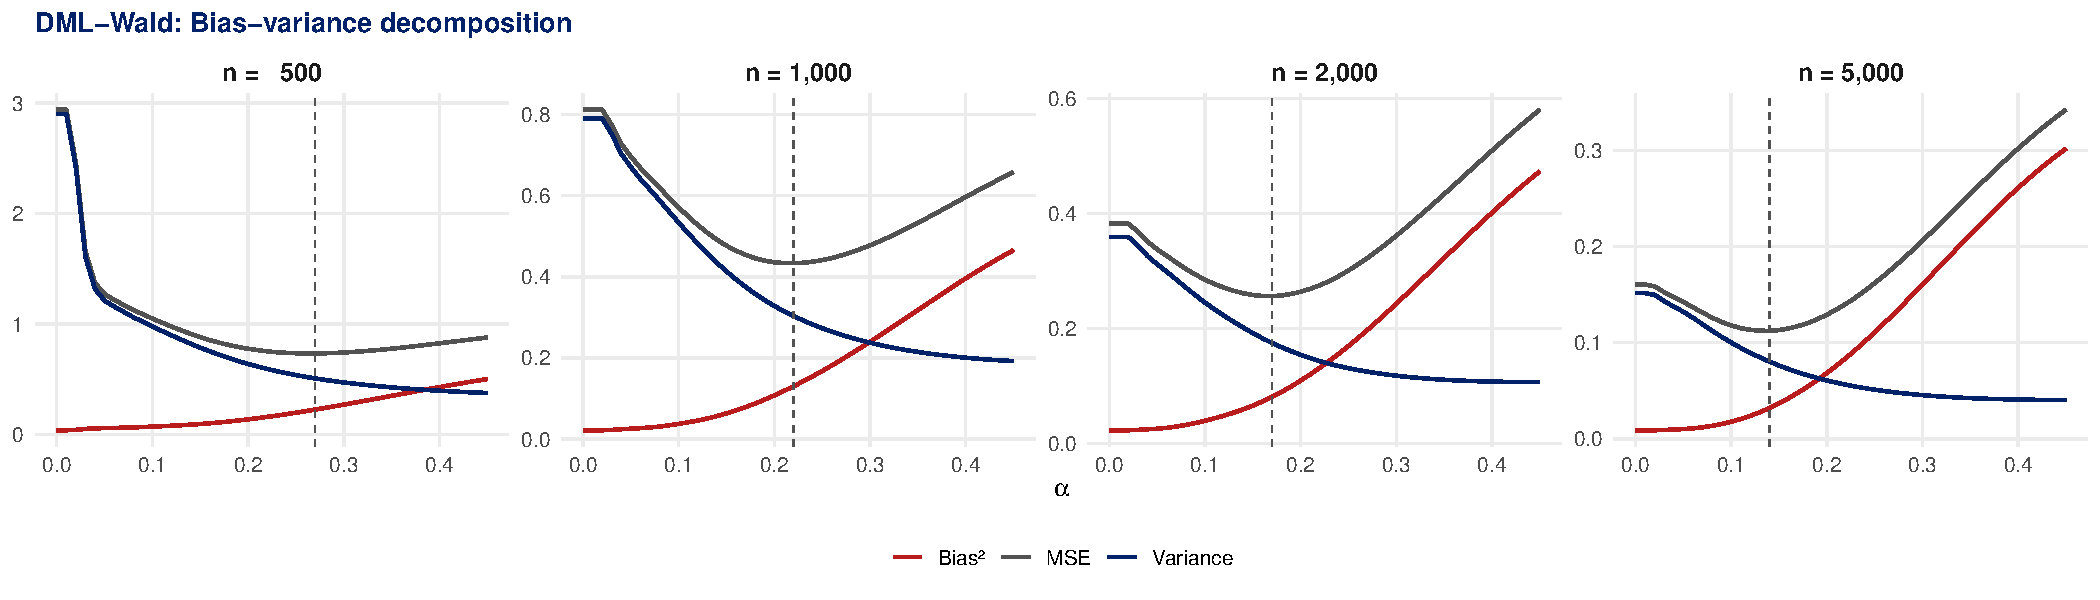
\includegraphics[width=\linewidth]{../output/figures/sim_trimming_wald.pdf}
    \caption[DML-Wald: bias-variance decomposition by trimming threshold]{DML-Wald: bias-variance decomposition as a function of the trimming threshold $\alpha$. Dashed vertical line marks the RMSE-minimizing $\alpha$ at each $n$. The data-driven rule of Section~\ref{sec:4c} selects $\hat\alpha$ near the RMSE-minimizing threshold without knowledge of the true parameter.}\label{fig:trim_wald}
\end{figure}

\section{Empirical Application}\label{sec:6}

I apply the estimators to Indonesia's INPRES school construction program, a canonical setting with imperfect compliance. School construction varied across districts and cohorts, but exposure to the program increased schooling without deterministically fixing completed education. \citet{duflo2001schooling} study this design with 2SLS, and \citet{fuzzy2018} recast it as a discrete DID-IV setting. This application is a useful test case for the DML estimators because the first-stage coefficient is small, the covariates are rich, and the propensity scores approach the boundary. I compare DML-Wald and DML-TC under symmetric trimming and the $\hat{\alpha}$-rule.

\subsection{Setting, data, and design}\label{sec:6_setup}

The INPRES program built more than 61{,}000 primary schools between 1973 and 1978, creating variation in school access across districts and cohorts. I use the 1995 Indonesian Intercensal Survey (SUPAS) microdata from \citet{duflo2001schooling}, pooling men and women with non-missing log hourly wage born in 1957--1962 (old cohort, $T=0$) or 1968--1972 (young cohort, $T=1$).

I adopt a binary district classifier $G^*$, which flags districts whose schooling distribution shifted upward between cohorts via a signed chi-squared test on the district's cohort-by-education table (Appendix~\ref{sec:app_classifier} provides details). \citet{fuzzy2018} also retain those districts with downward shifts by pooling $G^* \in \{-1, 0, +1\}$, and I exclude these 20 districts from the analysis. The final sample has $22{,}414$ observations in $201$ districts.

I compare two binary treatment thresholds, $D=\mathbf{1}\{\text{yeduc} \geq 6\}$ (primary completion) and $D=\mathbf{1}\{\text{yeduc} \geq 12\}$ (high-school completion), instrumented by the group-cohort interaction $G \times T$. The $p = 45$ covariate dictionary contains only individual-level regressors (sex, birth year interacted with cohort, Java, urban, and pairwise interactions). District-level covariates that mechanically predict $G^*$ are excluded because they would push $\hat e(X)$ to one and leave holdout cells empty. Appendix~\ref{sec:app_empirical} gives the full construction.


\subsection{Results}

Table~\ref{tab:empirical} reports the seven estimators under two trimming rules, separately for each binary threshold.

\begin{table}[h!]
    \centering
    \resizebox{\textwidth}{!}{\input{../output/tables/empirical_duflo.tex}}
    \caption[Returns to schooling from INPRES school construction]{Returns to schooling from INPRES school construction. Sample: both sexes with non-missing log hourly wage, cohorts 1957--1962 and 1968--1972, $G^* \in \{0, 1\}$, $N = 22{,}414$ ($201$ districts). Panel A uses $D = \mathbf{1}\{\text{yeduc} \geq 6\}$ (primary completion); Panel B uses $D = \mathbf{1}\{\text{yeduc} \geq 12\}$ (high-school completion). Outcome $Y$ is log hourly wage. Dictionary of $p = 45$ regressors from sex, birth-year dummies, Java, urban, and pairwise interactions (Appendix~\ref{sec:6c}). DML estimators use Lasso with $L = 5$-fold observation-level cross-fitting and the FSIF correction of Proposition~\ref{prop:2}. Superscript $s$ denotes symmetric trimming $\hat e(X) \in [0.10, 0.90]$ (Crump et al.\ 2009); superscript $\hat\alpha$ denotes the paper's one-sided data-driven rule of Conjecture~\ref{cor:onesided}, which returns $\hat\alpha = 0$ on this dictionary. Standard errors clustered at the district of birth. Bold marks the preferred estimate in each panel. Per-year CI rescales the per-complier interval by the threshold in years. Four-learner robustness in Appendix~\ref{sec:app_empirical}.}\label{tab:empirical}
\end{table}

\FloatBarrier
Two results organize the table. First, the FSIF correction systematically debiases the Lasso plug-in. Across the four plug-in–DML pairs (Wald$_X$ against DML-Wald and TC$_X$ against DML-TC, at each threshold), the plug-in overstates the return to schooling by between $0.2$ and $0.8$ standard errors, and the sign is always positive. At primary completion TC$_X = 1.27$ drops to DML-TC $= 1.06$ and Wald$_X = 2.20$ drops to DML-Wald $= 2.07$; the high-school corrections are smaller but point the same way. Cluster-robust intervals tighten by $6$ to $8\%$ at primary completion and are essentially unchanged at high school. The heterogeneity story between the two estimands is secondary. The DML-Wald and DML-TC gap of $2.07$ versus $1.06$ at primary completion cannot be blamed on a weak instrument (first-stage $F = 59.8$, and $48.2$ at high school) and is consistent with heterogeneous returns across districts with different INPRES exposure. DML-TC is preferred because it replaces the stronger stable-conditional-treatment-effects restriction in Assumption~\ref{ass:5} with the within-treatment-status common-trends restriction in Assumption~\ref{ass:4prime}.

Second, the trimming rule is inactive here. The $\hat\alpha$-rule returns $\hat\alpha = 0$, and the DML point estimates remain stable as $\alpha$ is pushed to $0.20$ (Appendix Figure~\ref{fig:sensitivity_app}). The propensity distribution is interior with support $[0.53, 0.91]$ and no mass near the boundary (Appendix Figure~\ref{fig:propensity_app}), which is what delivers the insensitivity. The $p = 45$ dictionary is deliberately built from individual-level regressors only, with no district aggregates that would mechanically pin down $G^*$.\footnote{In a companion exercise using a $p = 141$ dictionary that adds district-level covariates, $\hat e(X)$ saturates at the upper boundary, the $\hat\alpha$-rule binds at $\hat\alpha > 0$, and the DML-TC point estimate remains within one standard error of the $p = 45$ result. Replication code is available at \url{https://github.com/andres-mena/DID_LATE}.}

\section{Conclusion}\label{sec:7}

This paper recasts the fuzzy DID design of \citet{fuzzy2018} as a debiased machine-learning problem. The Wald-DID and time-corrected estimands are rewritten as unconditional moments and augmented with closed-form first-step influence functions, yielding orthogonal scores whose Riesz representers are propensity-weighted cell indicators. DML-Wald and DML-TC inherit $\sqrt{n}$-consistency and asymptotic normality under a standard product-rate condition and achieve the semiparametric efficiency bound up to normalization. A data-driven one-sided trimming rule selects the threshold that minimizes a sample analog of the estimator's asymptotic variance relative to the squared first stage. The rule discards only observations whose probability of belonging to the treated group is close to one and preserves the first-stage information that symmetric rules waste.

Two lessons run through the simulations and the INPRES application. Orthogonality, not the choice of learner, drives the gains. Across Lasso, Ridge, elastic-net, and random forests DML-TC estimates agree within $0.05$ log points per year of schooling at both margins, while Monte Carlo bias falls by a factor of three to five relative to Lasso plug-ins. When the first-stage coefficient is small, the Wald ratio amplifies noise and DML-TC becomes the operational estimator. At the INPRES primary-completion margin DML-TC corrects an upward bias in the Lasso plug-in and tightens the cluster-robust confidence interval. Reporting both scores serves as a specification check. Agreement is reassuring, and disagreement signals that the conditional stability of treatment effects may fail.

The FSIF construction transfers to richer designs. Three extensions follow naturally: staggered adoption with multiple periods \citep{callaway2023ddml}, panel data with individual fixed effects, and district-level treatment with cluster-level cross-fitting. The cluster case is treated in Remark~\ref{rem:cluster} following \citet{chiang2022multiway} and \citet{belloni2017program}; the first two are left for future work. The one-sided optimality of the trimming rule is likewise stated as a conjecture that tracks the population tilting measure (Appendix~\ref{sec:app_trimming}); a formal treatment with the estimated measure is the natural next step.


\newpage
\bibliographystyle{aea}
\bibliography{biblio}

\newpage
\appendix
\renewcommand{\thesection}{\Alph{section}}
\renewcommand{\thesubsection}{\Alph{section}.\arabic{subsection}}
\renewcommand{\thefigure}{\thesection.\arabic{figure}}
\renewcommand{\thetable}{\thesection.\arabic{table}}

\section{Simulations: Additional results}\label{sec:app_sim}

\begin{table}[H]
    \centering
    \input{../output/tables/sim_main.tex}
    \caption[Monte Carlo simulation: main results]{Monte Carlo simulation, $M = 1{,}000$ replications, true $\Delta = 1$, nonlinear DGP, Lasso on $p = 100$ covariates ($p_0 = 20$ signal, $80$ noise). DML estimators use $L = 5$-fold cross-fitting with the data-driven one-sided $\hat\alpha$-rule of Conjecture~\ref{cor:onesided} (Section~\ref{sec:4c}); TC cell propensities $\pi_{dgt}$ trimmed to $[0.01, 0.99]$. Bold marks the best performer per metric per panel. SE/SD is the ratio of the mean estimated standard error to the Monte Carlo standard deviation (1.000 indicates perfect calibration).}\label{tab:main_sim}
\end{table}

\begin{table}[H]
    \centering
    \input{../output/tables/sim_ml_comparison.tex}
    \caption[DML estimators with alternative first-step methods]{DML estimators with alternative first-step methods. Lasso uses $p = 100$ covariates with $L_1$ regularization. Random Forest uses 500 trees with $\lfloor p/3 \rfloor$ variables per split. Neural Network uses a single hidden layer with 5 units and weight decay 0.01. Propensity scores estimated via logit-Lasso in all cases. $M = 1{,}000$ replications, $L = 5$-fold cross-fitting, data-driven trimming.}\label{tab:ml_comparison}
\end{table}

\begin{table}[H]
    \centering
    \small
    \input{../output/tables/sim_trim_rule_summary.tex}
    \caption[Data-driven trimming vs.\ Crump et al.\ (2009) symmetric rule]{Data-driven one-sided trimming versus the Crump et al.\ (2009) symmetric $[0.10, 0.90]$ rule. Monte Carlo bias, standard deviation, RMSE, and 95\% coverage for DML-Wald and DML-TC under each rule, pooled across $M = 1{,}000$ replications. Superscript $\hat\alpha$ denotes the paper's one-sided data-driven rule (Conjecture~\ref{cor:onesided}); superscript $s$ denotes symmetric $[0.10, 0.90]$ trimming. The last column reports the average share of observations dropped by each rule. The data-driven rule selects $\hat\alpha \approx 0.20$ at moderate $n$, trims more aggressively at the upper tail than the symmetric rule, and reduces RMSE at every sample size. DML-TC is largely insensitive to the rule.}\label{tab:trim_rule}
\end{table}

\section{Empirical Application: Additional Results}\label{sec:app_empirical}

\subsection{Classifier construction}\label{sec:app_classifier}

The binary group indicator $G^*_d$ is constructed separately for each district $d$ in three steps, following \cite[][Section 5.2]{fuzzy2018}.

\paragraph{Step 1: Contingency table.} Cross-tabulate individuals in district $d$ by years of schooling and cohort into cell counts $n_{d,k,c}$, where $k \in \{0, 1, \ldots, 18\}$ indexes \texttt{yeduc} and $c \in \{0, 1\}$ indexes the young-cohort indicator.

\paragraph{Step 2: Chi-squared test of independence.} The null is that \texttt{yeduc} and \texttt{young} are independent in district $d$, which means the schooling distribution is the same in the old and young cohorts. The test statistic is
\begin{equation*}
\chi^2_d = \sum_{k,\,c} \frac{(n_{d,k,c} - E_{d,k,c})^2}{E_{d,k,c}}, \qquad E_{d,k,c} = \frac{n_{d,k,\cdot}\,n_{d,\cdot,c}}{n_{d,\cdot,\cdot}},
\end{equation*}
which has approximately a $\chi^2$ distribution with degrees of freedom equal to one less than the number of nonempty \texttt{yeduc} rows. Let $p_d$ denote the p-value. Rejecting $H_0$ flags district $d$ as having a cohort-level shift in the schooling distribution.

\paragraph{Step 3: Sign the rejection.} The test is two-sided, so \citeauthor{fuzzy2018} sign each rejection by the direction of the change in mean schooling between cohorts,
\begin{equation*}
G^*_d = \begin{cases}
+1 & p_d < 0.5 \text{ and } \overline{\text{yeduc}}_{d,\text{young}} > \overline{\text{yeduc}}_{d,\text{old}}, \\
-1 & p_d < 0.5 \text{ and } \overline{\text{yeduc}}_{d,\text{young}} < \overline{\text{yeduc}}_{d,\text{old}}, \\
\phantom{+}0 & p_d \geq 0.5.
\end{cases}
\end{equation*}

\paragraph{Interpretation.} $G^*_d = +1$ marks districts where INPRES plausibly shifted schooling upward, which are the treatment group in this paper. $G^*_d = 0$ marks districts with no detectable cohort shift, the control group. $G^*_d = -1$ marks districts where schooling shifted downward for reasons unrelated to INPRES. This paper drops $G^*_d = -1$ districts because Theorem~\ref{thm:1} is stated for binary $G$. The threshold $p_d < 0.5$ is a classification cutoff, not a conventional significance test. It is chosen to label every district as one of $\{-1, 0, +1\}$ rather than to provide inference on whether a shift occurred.

\subsection{Sample and classifier}\label{sec:app_sample}

I use the 1995 Indonesian Intercensal Survey (SUPAS) microdata from \citet{duflo2001schooling}. The sample pools both sexes with non-missing log hourly wage, born in 1957--1962 (old cohort, $T=0$) or 1968--1972 (young cohort, $T=1$). Years of schooling is top-coded at $18$ (recoding $19 \to 18$ to match the \citeauthor{fuzzy2018} replication). The outcome $Y$ is log hourly wage and the classifier $G^*$ is the chi-squared test on the full $\text{yeduc} \times \text{young}$ contingency table at threshold $p < 0.5$, signed by the change in mean years of schooling. The paper's theorem is stated for binary $G$, so I restrict to $G^* \in \{0, 1\}$ and drop the $G = -1$ districts. Table~\ref{tab:classifier} compares classifier counts to \cite{duflo2001schooling} and \cite{fuzzy2018}.

\begin{table}[H]
    \centering
    \small
    \input{../output/tables/empirical_classifier.tex}
    \caption[District classifier comparison]{District classifier comparison. \cite{duflo2001schooling} uses continuous INPRES intensity as an instrument and has no binary $G^*$. \cite{fuzzy2018} Table~3 reports counts $97/64/123$; ours are $96/67/127$, within $\pm 4$ districts due to boundary drift between R's \texttt{chisq.test} and Stata's \texttt{tab2, chi2}. \citeauthor{fuzzy2018} pool $G^* \in \{-1, 0, +1\}$ via a mirror Wald formula and report on the full 284-district sample. This paper's theorem handles binary $G$, so I restrict to $G^* \in \{0, 1\}$, which gives $N = 22{,}414$ observations in $201$ districts.}\label{tab:classifier}
\end{table}

\subsection{Covariate dictionary and excluded variables}\label{sec:6c}

The dictionary contains $p = 45$ individual-level regressors: sex, birth year interacted with cohort, Java residence at birth, urban residence at birth, and their pairwise interactions. These vary within both $G = 0$ and $G = 1$ districts and keep $\hat e(X)$ strictly interior on the full sample (Figure~\ref{fig:propensity_app}). Estimation uses observation-level cross-fitting with $L = 5$ folds and cluster-robust standard errors at the district of birth following Remark~\ref{rem:cluster}.

District-level statistics that summarize the cohort-by-education distribution (mean education of older cohorts, 1971 enrollment rate, 1971 children population) are excluded because they pin $\Pr(G = 1 \mid X) \in \{0, 1\}$ by construction, driving $\hat e(X)$ to the boundary and emptying holdout cells after trimming. Pre-INPRES district variables correlated with the INPRES allocation rule (program intensity, 1971 population density, water and sanitation spending) are also excluded because conditioning on them absorbs the first-stage variation that identifies the LATE.

\subsection{Descriptive statistics and diagnostics}\label{sec:app_descriptives}

\begin{table}[H]
    \centering
    \input{../output/tables/empirical_balance.tex}
    \caption[Descriptive statistics by group-time cell]{Descriptive statistics by group-time cell. $G=1$ districts experienced a significant cohort shift in the education distribution with rising schooling; $G=0$ districts did not. $T=0$ is the old cohort (1957--1962, unexposed to INPRES), $T=1$ the young cohort (1968--1972, exposed). $Y$ is log hourly wage; $D = \mathbf{1}\{\text{years of schooling} \geq 6\}$. District-level covariates are from 1971 census data. Standard deviations in parentheses.}\label{tab:balance}
\end{table}

\begin{figure}[H]
    \centering
    \begin{subfigure}[b]{0.48\linewidth}
        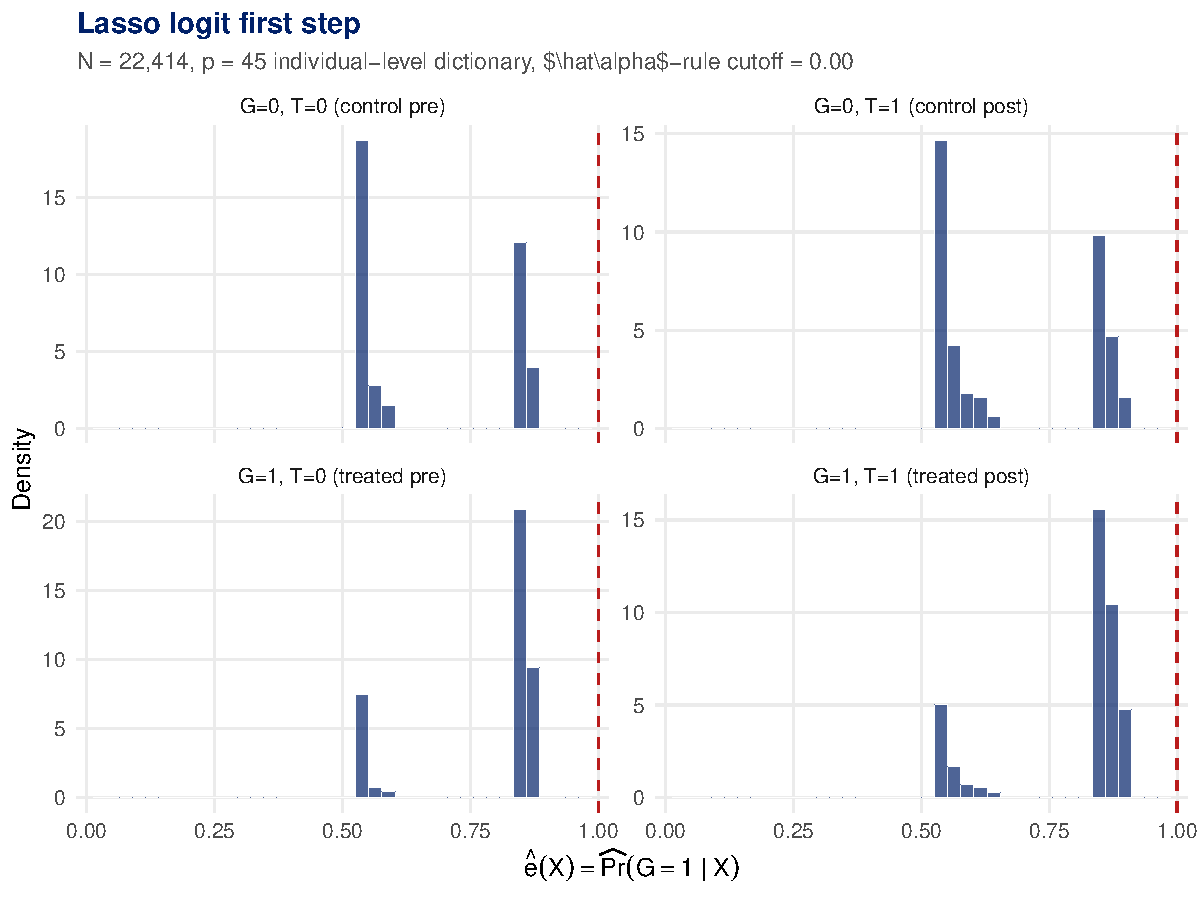
\includegraphics[width=\linewidth]{../output/figures/empirical_propensity_lasso.pdf}
        \caption{Logit-Lasso first step.}\label{fig:propensity_lasso}
    \end{subfigure}
    \hfill
    \begin{subfigure}[b]{0.48\linewidth}
        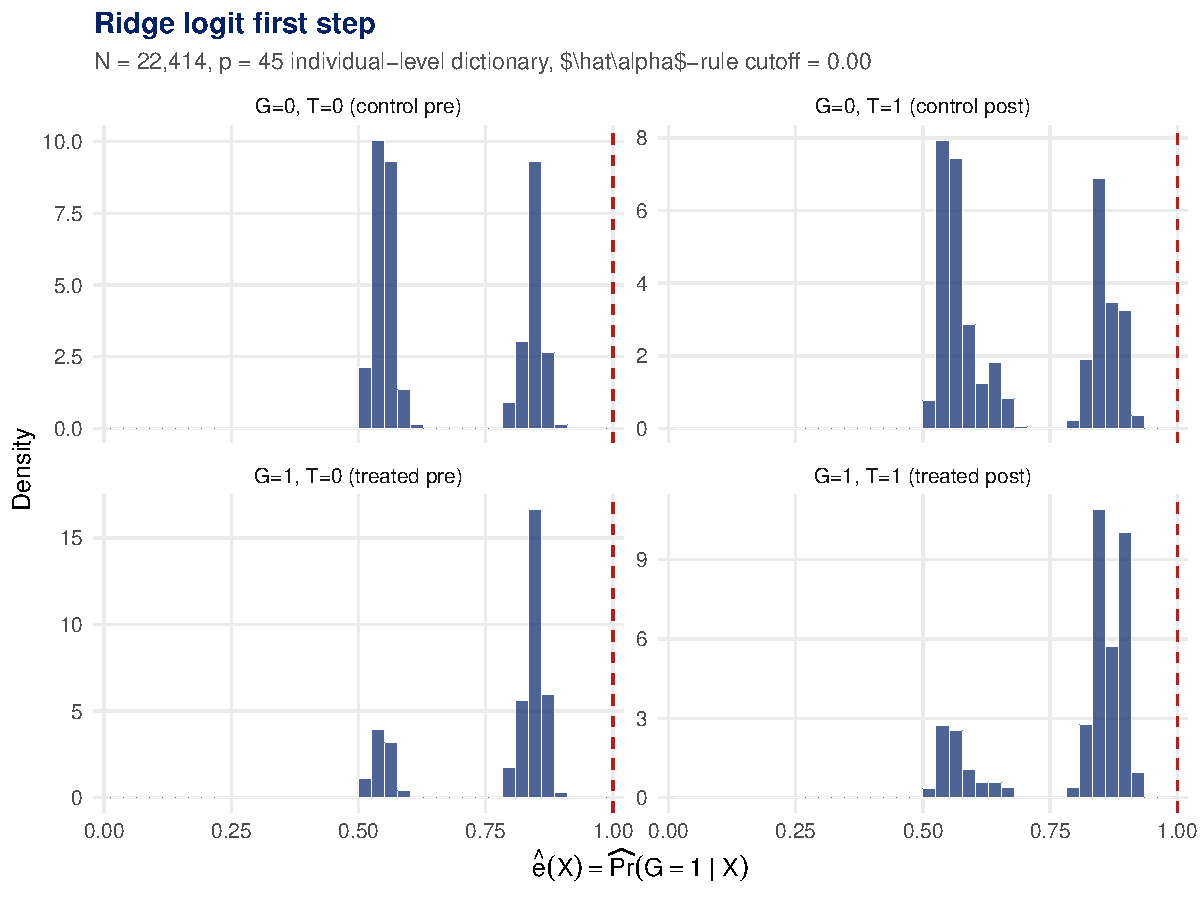
\includegraphics[width=\linewidth]{../output/figures/empirical_propensity_ridge.pdf}
        \caption{Logit-Ridge first step.}\label{fig:propensity_ridge}
    \end{subfigure}
    \caption[Propensity score distribution by $(G,T)$ cell]{Distribution of $\hat e(X) = \hat{\Pr}(G=1 \mid X)$ by $(G,T)$ cell on the $p=45$ individual-level dictionary ($N = 22{,}414$). Both Lasso and Ridge produce interior propensities with no mass at the boundary. Lasso range $[0.53, 0.91]$ with mean $0.77$ and SD $0.14$; Ridge range $[0.51, 0.91]$ with mean $0.77$ and SD $0.14$. The share above $0.9$ is $1\%$ under Lasso and $6\%$ under Ridge; below $0.1$ is $0\%$ under both. The $\hat\alpha$-rule of Conjecture~\ref{cor:onesided} returns $\hat\alpha = 0$ under both learners, so the dashed line at $1 - \hat\alpha = 1$ coincides with the right edge and the full sample is retained.}\label{fig:propensity_app}
\end{figure}

\subsection{Sensitivity to trimming and learner choice}\label{sec:app_sensitivity}

\begin{figure}[H]
    \centering
    \begin{subfigure}[b]{0.48\linewidth}
        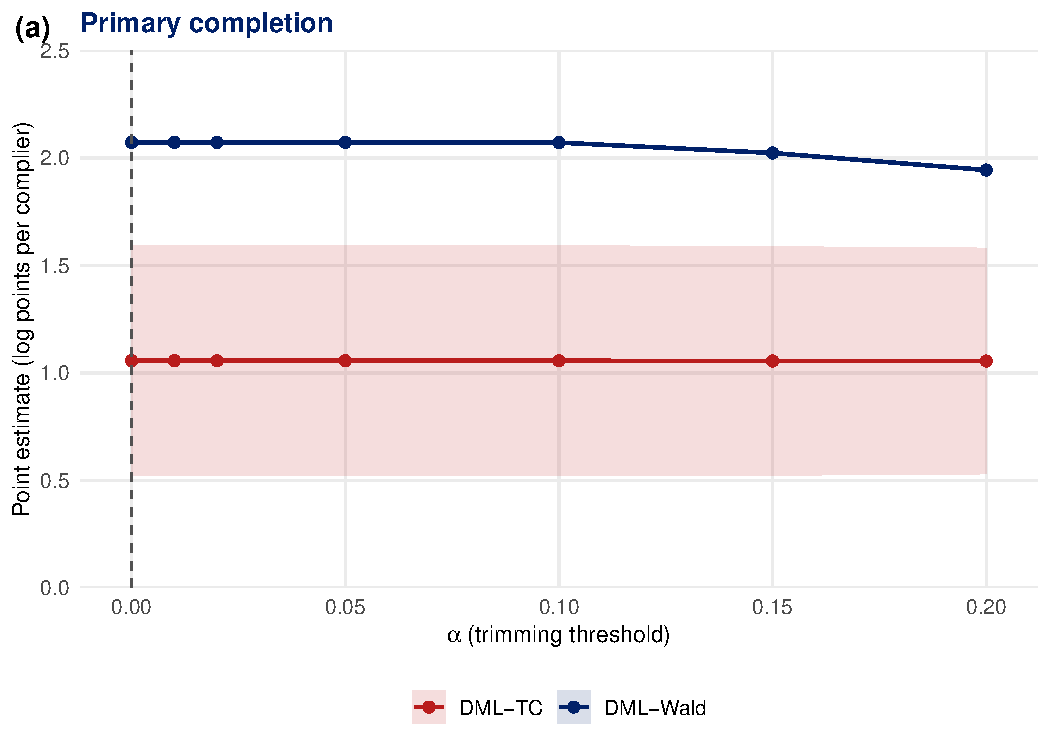
\includegraphics[width=\linewidth]{../output/figures/empirical_sensitivity_primary.pdf}
        \caption{Primary completion ($D \ge 6$).}\label{fig:sensitivity_primary}
    \end{subfigure}
    \hfill
    \begin{subfigure}[b]{0.48\linewidth}
        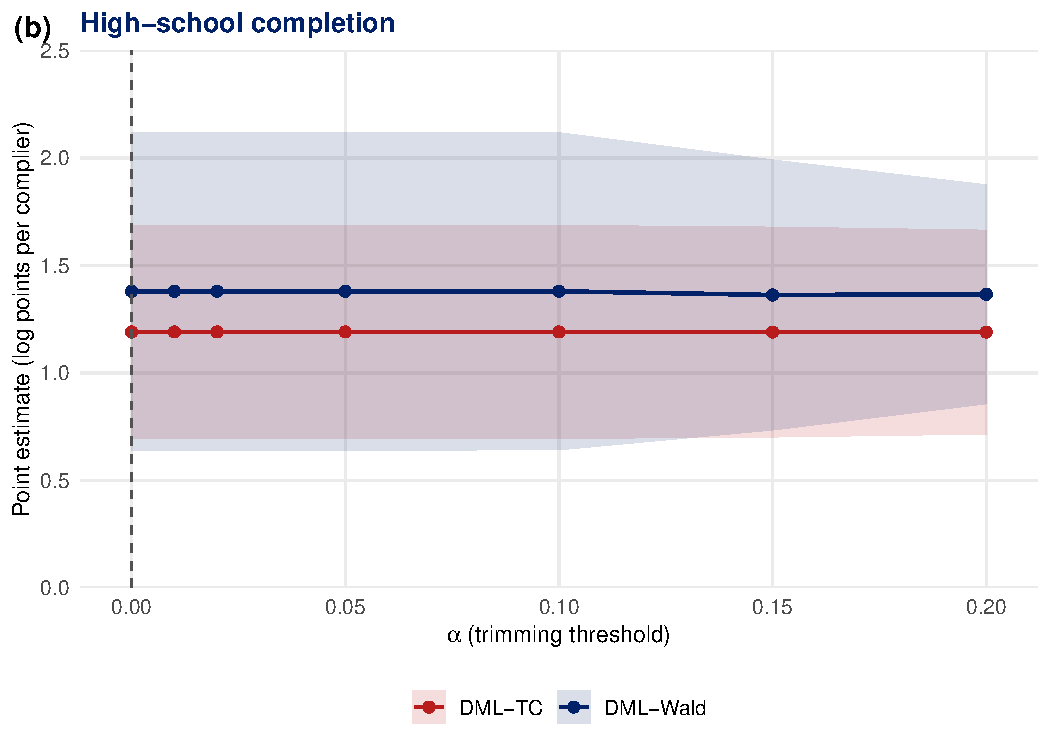
\includegraphics[width=\linewidth]{../output/figures/empirical_sensitivity_highschool.pdf}
        \caption{High-school completion ($D \ge 12$).}\label{fig:sensitivity_highschool}
    \end{subfigure}
    \caption[Sensitivity to one-sided trimming threshold]{DML-Wald and DML-TC point estimates as a function of the one-sided trimming threshold $\alpha \in [0, 0.20]$. DML-TC is flat over the full range at both margins; DML-Wald drifts but its standard error bands remain wide.}\label{fig:sensitivity_app}
\end{figure}

\begin{table}[H]
    \centering
    \small
    \input{../output/tables/empirical_4learner.tex}
    \caption[DML estimates across four first-step learners]{DML-Wald and DML-TC point estimates (cluster-robust SE in parentheses) at both treatment margins across four first-step learners. All columns use the $\hat\alpha$-rule, which returns $\hat\alpha = 0$ on the $p=45$ dictionary. DML-TC estimates agree within $0.4$ log points across learners at the primary margin and within $0.3$ at the high-school margin. DML-Wald shows more dispersion at the primary margin, reflecting the fragility of the Wald ratio under a modest first stage ($\mathrm{DID}_D = 0.088$).}\label{tab:empirical_4learner}
\end{table}

\section{Proofs}

This appendix proves the paper's original results. The identification assumptions and the underlying identification result of \citet{fuzzy2018} are reproduced in Appendix~\ref{sec:app_cdh_reference} for reader convenience.

\begin{center}
\small
\begin{tabular}{llcl}
\toprule
Result & Statement & Location & Proof \\
\midrule
Proposition~\ref{prop:1} & Identifying moments for Wald-DID and TC & §\ref{sec:3a} & Appendix~\ref{sec:app_proof_prop1} \\
Proposition~\ref{prop:2} & Closed-form first-step influence functions & §\ref{sec:3b} & Appendix~\ref{sec:app_proof_prop2} \\
Proposition~\ref{prop:3} & Local robustness of $\psi^{wald}$ and $\psi^{tc}$ & §\ref{sec:3c} & Appendix~\ref{sec:app_proof_prop3} \\
Theorem~\ref{thm:1} & $\sqrt{n}$-consistency and asymptotic normality & §\ref{sec:3e} & Appendix~\ref{sec:app_proofs_thm1} \\
Proposition~\ref{prop:4} & Semiparametric efficiency & §\ref{sec:3e} & Appendix~\ref{sec:app_proofs_prop4} \\
\bottomrule
\end{tabular}
\end{center}

\subsection{Proof of Proposition~\ref{prop:1}: Identifying Moments}\label{sec:app_proof_prop1}
\begin{propproof}

\noindent \\
\textit{At the true nuisance vectors, the pointwise moments in \eqref{eq:5} and \eqref{eq:6} generate the same zero restrictions as the centered estimands in \eqref{eq:Wdid} and \eqref{eq:Wtc}. Therefore, under the corresponding identification assumptions, both moment functions identify the same target $\Delta$.}

\medskip
\noindent\textbf{Proof.} I show that $E[g^j(W,\gamma^j_0,\theta)]=0$ is equivalent to the corresponding centered estimand being zero, then apply the identification results of \cite{fuzzy2018}.

\medskip
\noindent\textit{Wald case.} At the true nuisance vector, for any $\theta$,
\begin{align*}
    g^{wald}(W,\gamma^{wald}_0,\theta) &= \frac{GT}{p_{11}}\big[(Y-m^Y_{10}(X)-m^Y_{01}(X)+m^Y_{00}(X))- (D-m^D_{10}(X) \\
    &\quad -m^D_{01}(X)+m^D_{00}(X))\theta\big] \\
     &= \frac{GT}{p_{11}}[DID_Y(X)-DID_D(X)\theta].
\end{align*}
Taking expectations on both sides, recalling that $E[GT]=p_{11}=\Pr(G=1,T=1)$, and using linearity of expectations and the definition of conditional expectation, this gives:
\begin{align*}
    E[g^{wald}(W,\gamma^{wald}_0,\theta)] &= E\left[\frac{GT}{p_{11}}(DID_Y(X)-DID_D(X)\theta)\right]  \\
    &= E\left[DID_Y(X)|G=1,T=1\right] - E\left[DID_D(X)|G=1,T=1\right]\theta.
\end{align*}
Since the denominator in $W^{DID}$ is nonzero,
\begin{align*}
    \frac{E[g^{wald}(W,\gamma^{wald}_0,\theta)]}
    {E\left[DID_D(X)|G=1,T=1\right]}
    &= W^{DID} - \theta.
\end{align*}
Therefore $E[g^{wald}(W,\gamma^{wald}_0,\theta)]=0$ if and only if $W^{DID}-\theta=0$. Under the Wald-DID identification assumptions, \citet{fuzzy2018} gives $W^{DID}=\Delta$.

\noindent\textit{TC case.} The same calculation gives, at the true nuisance vector and for any $\theta$,
\begin{align*}
    E[g^{tc}(W,\gamma^{tc}_0,\theta)]
    &= E\left[Y-m^Y_{10}(X)-m^D_{10}(X)\delta_1(X)-(1-m^D_{10}(X))\delta_0(X)\mid G=1,T=1\right] \\
    &\quad - E\left[D-m^D_{10}(X)\mid G=1,T=1\right]\theta.
\end{align*}
Since the denominator in $W^{TC}$ is nonzero,
\[
    E[g^{tc}(W,\gamma^{tc}_0,\theta)]=0
    \quad\Longleftrightarrow\quad
    W^{TC}-\theta=0.
\]
Under the TC identification assumptions, \citet{fuzzy2018} gives $W^{TC}=\Delta$. $\square$

\end{propproof}

\subsection{Proof of Proposition~\ref{prop:2}: First-Step Influence Functions}\label{sec:app_proof_prop2}\label{sec:app_fsif}
\begin{propproof}

\noindent \\
\textit{For $j\in\{\text{wald},\text{tc}\}$, let $\mathcal{M}^j(\gamma^j,\theta)=E[g^j(W,\gamma^j,\theta)]$. The first-step influence function of $\mathcal{M}^j$ with respect to $\gamma^j$ is $\phi^j(W,\gamma^j,\alpha^j,\theta)=\sum_{k=1}^{K_j}\alpha^j_k(W)(R^j_k-\gamma^j_k(X))$. The closed-form Riesz representers are given by Equations~\ref{eq:fsif_wald_alpha_app}--\ref{eq:fsif_tc_alpha2_app}, and the element-by-element expressions for $\phi^{wald}$ and $\phi^{tc}$ are Equations~\ref{eq:8_app}--\ref{eq:9_app}.}

\medskip
\noindent\textbf{Proof.} I follow the pathwise derivative framework of \cite{ichimura2022influence} to derive the FSIF by computing the Gateaux derivative of $\mathcal{M}^j(\gamma^j(F),\theta)$ along smooth paths $F_\tau = (1-\tau)F_0 + \tau H$. Since $g^{wald}$ is additively separable in its $K=6$ nuisance functions, the FSIF decomposes as a sum of component-wise FSIFs by Ichimura and Newey (2022, Section 5).

\medskip
\noindent\textit{Pathwise setup and cell weights.} For a path $F_\tau = (1-\tau)F_0 + \tau H$, the first-step influence function $\phi(W,\gamma,\alpha,\theta)$ associated with the moment $g(W,\gamma,\theta)$ satisfies
\begin{equation}\label{eq:fsif_def_app}
    \frac{\partial}{\partial \tau}E[g(W,\gamma(F_{\tau}),\theta)]\bigg|_{\tau=0}
    = \int \phi(w,\gamma_0,\alpha_0,\theta)\,H(dw),
    \qquad E[\phi(W,\gamma_0,\alpha_0,\theta)] = 0,
    \qquad E[\phi^2] < \infty.
\end{equation}
The Riesz representers below express this derivative as a weighted residual. Define $\pi_{gt}(X)=\Pr(G\!=\!g,T\!=\!t\mid X)$ and $\pi_{dgt}(X)=\Pr(D\!=\!d,G\!=\!g,T\!=\!t\mid X)$. For any relevant $(G,T)$ or $(D,G,T)$ cell $c$, set
\begin{equation}\label{eq:cellweight_app}
    \rho_c(W)=\frac{\mathbf{1}\{W\in c\}\,\pi_{11}(X)}{\pi_c(X)\,p_{11}}.
\end{equation}
The factor $\rho_c$ selects observations in cell $c$ and reweights them toward the target cell $(G,T)=(1,1)$.

\medskip
\noindent\textit{Closed-form representers.} Differentiating \eqref{eq:5} with respect to $\gamma^{wald}=\{m^R_{gt}\}_{R\in\{Y,D\},(g,t)\neq(1,1)}$ yields
\begin{equation}\label{eq:fsif_wald_alpha_app}
    \alpha^{wald}_{m^R_{gt}}(W)=\lambda^R_{gt}\,\rho_{gt}(W),
\end{equation}
where
\begin{equation*}
    \lambda^Y_{10}=\lambda^Y_{01}=-1,\quad \lambda^Y_{00}=1,
    \qquad
    \lambda^D_{10}=\lambda^D_{01}=\theta,\quad \lambda^D_{00}=-\theta.
\end{equation*}
Differentiating \eqref{eq:6} with respect to $\gamma^{tc}=\{m^Y_{10},m^D_{10},\mu^Y_{d0t}\}_{d,t\in\{0,1\}}$ yields
\begin{align}
    \alpha^{tc}_{m^Y_{10}}(W)&=-\rho_{10}(W), \label{eq:fsif_tc_alpha1_app}\\
    \alpha^{tc}_{m^D_{10}}(W)&=(\delta_0(X)-\delta_1(X)+\theta)\rho_{10}(W), \label{eq:fsif_tc_alpha1b_app}\\
    \alpha^{tc}_{\mu^Y_{d0t}}(W)&=(-1)^t q_d(X)\rho_{d0t}(W), \label{eq:fsif_tc_alpha2_app}
\end{align}
where $q_1(X)=m^D_{10}(X)$ and $q_0(X)=1-m^D_{10}(X)$.

\medskip
\noindent\textit{Explicit FSIFs.} Substituting \eqref{eq:fsif_wald_alpha_app} and \eqref{eq:fsif_tc_alpha1_app}--\eqref{eq:fsif_tc_alpha2_app} into $\phi^j=(\alpha^j)^\top(R^j-\gamma^j)$ gives
\begin{equation}\label{eq:8_app}
\begin{aligned}
    \phi^{wald} = & -\frac{G(1-T)\pi_{11}(X)}{\pi_{10}(X)p_{11}} \Big(Y-m^Y_{10}(X)- (D-m^D_{10}(X))\theta\Big) \\
    & - \frac{(1-G)T\pi_{11}(X)}{\pi_{01}(X)p_{11}}\Big(Y-m^Y_{01}(X)- (D-m^D_{01}(X))\theta\Big) \\
    & + \frac{(1-G)(1-T)\pi_{11}(X)}{\pi_{00}(X)p_{11}} \Big(Y-m^Y_{00}(X)- (D-m^D_{00}(X))\theta\Big),
\end{aligned}
\end{equation}
and
\begingroup\small
\begin{equation}\label{eq:9_app}
\begin{aligned}
    \phi^{tc} = & -\frac{G(1\!-\!T)\pi_{11}}{\pi_{10}\,p_{11}} \Big(Y\!-\!m^Y_{10}\!-\! (D\!-\!m^D_{10})(\delta_0\!-\!\delta_1\!+\!\theta)\Big) \\
    & - m^D_{10}\frac{\pi_{11}}{p_{11}}\bigg(\frac{D(1\!-\!G)T}{\pi_{101}} (Y\!-\!\mu^Y_{101}) - \frac{D(1\!-\!G)(1\!-\!T)}{\pi_{100}}(Y\!-\!\mu^Y_{100})\bigg) \\
    & - (1\!-\!m^D_{10})\frac{\pi_{11}}{p_{11}}\bigg(\frac{(1\!-\!D)(1\!-\!G)T}{\pi_{001}} (Y\!-\!\mu^Y_{001}) - \frac{(1\!-\!D)(1\!-\!G)(1\!-\!T)}{\pi_{000}}(Y\!-\!\mu^Y_{000})\bigg).
\end{aligned}
\end{equation}
\endgroup
The rest of the proof verifies these representers from the pathwise derivative.

\medskip
\noindent\textit{Wald case.}

Since $g^{wald}$ depends on $K = 6$ nuisance functions $\gamma^{wald} = (m^Y_{10}, m^Y_{01}, m^Y_{00}, m^D_{10}, m^D_{01}, m^D_{00})$ and is additively separable in each, the FSIF decomposes as a sum of component-wise FSIFs (Ichimura and Newey 2022, Section 5):\\

$$ \phi^{wald}(W, \gamma^{wald}, \alpha^{wald}, \theta) = \sum_{k=1}^{6} \phi_k(W, \gamma_k, \alpha_k, \theta) $$\\

For each component $\gamma_k(X) = E[R_k | G = g_k, T = t_k, X]$, the key observation is that $g^{wald}$ is \textit{linear} in $\gamma_k$. This means Assumptions 1--2 of \cite{ichimura2022influence} are trivially satisfied: the coefficient of $\gamma_k(X)$ in $E[g^{wald}]$ yields $v_{m,k}(X)$ directly, and the residual $\rho_k(W, \gamma_k) = \mathbf{1}_{[G=g_k, T=t_k]}(R_k - \gamma_k(X))$ gives $v_{\rho,k}(X) = -\pi_{g_k t_k}(X)$. The Riesz representer is therefore $\alpha_k(X) = v_{m,k}(X) / \pi_{g_k t_k}(X)$, and the component-wise FSIF is $\phi_k = \alpha_k(X) \rho_k(W, \gamma_k)$.\\

The vector of nuisance functions for the $g^{wald}(W,\gamma^{wald}(F_{\tau}),\theta)$ moment function on equation \ref{eq:5} is:\\

$$\gamma^{wald}(F_{\tau})=[m^Y_{10}(F_{\tau}),m^Y_{01}(F_{\tau}),m^Y_{00}(F_{\tau}),m^D_{10}(F_{\tau}),m^D_{01}(F_{\tau}),m^D_{00}(F_{\tau})]$$\\

Since $g^{wald} = (GT/p_{11})[\ldots]$ and $E[GT/p_{11}|X] = \pi_{11}(X)/p_{11}$, the functional derivative of $E[g^{wald}]$ with respect to each nuisance function $\gamma_k(X)$ at point $X$ carries the factor $\pi_{11}(X)/p_{11}$. The gradient is:

$$ \nabla \mathbf{G(\gamma^{wald})}' = \frac{\pi_{11}(X)}{p_{11}}[-1,-1,1,\theta,\theta,-\theta] $$

where the signs for $m^D_{gt}$ components are positive because $g^{wald}$ contains $-(D - m^D_{10} - m^D_{01} + m^D_{00})\theta$, so $\partial/\partial m^D_{10} = +\theta \cdot \pi_{11}/p_{11}$.

The computation of the influence functions $\mathbb{IF}(\gamma^{wald}(F_{\tau}))$ follows the pathwise derivative framework of \cite{ichimura2022influence}. For each nuisance function $\gamma_k(X) = E[R_k | G=g_k, T=t_k, X]$, the influence function is the Gateaux derivative of the conditional expectation functional along the path $F_\tau = (1-\tau)F_0 + \tau H$. By Proposition 1 of \cite{ichimura2022influence}, this yields the following for the $(G=1,T=0)$ component:

\begin{align}\label{proof:2a}
    \mathbb{IF}(E_{F_{\tau}}[Y|G=1,T=0,X])  &= \frac{\partial}{\partial \tau}\sum_{X,Y}Y p_{\tau}(Y|1,0,X)\bigg|_{\tau=0} &\notag \\
    &= \sum_{X,Y}Y \frac{\partial}{\partial \tau} p_{\tau}(Y|G=1,T=0,X)\bigg|_{\tau=0}
\end{align}\\

Define the event $A=G(1-T)=\mathds{1}_{[G=1,T=0]}$, the subprocess $Z=(Y,G,T,X)$ with pmf $p_{\tau}(Z)=p_{\tau}(Y,G,T,X|D=0)p_{\tau}(D=0)+p_{\tau}(Y,G,T,X|D=1)p_{\tau}(D=1)$ , and note that for the submodel $p_{\tau}(Z)$:

\begin{align*}
    p_{\tau}(Y|G=1,T=0,X)&=\frac{p_{\tau}(Z)}{p_{\tau}(A,X)} &= \frac{(1-\tau) p_0(Z) + \tau \mathds{1}_{[Z=z]}}{(1-\tau) p_0(A, \omega) + \tau \mathds{1}_{[A=a,Z=z]}}  \\
    p_{\tau}(A,X)&=\frac{p_{\tau}(A,X)}{p_{\tau}(X)} &=\frac{(1-\tau) p_0(A,X) + \tau \mathds{1}_{[(A=a,X=x)]}}{(1-\tau) p_0(X) + \tau \mathds{1}_{[X=x]}}  \\
    p_{\tau}(X)&=(1-\tau) p_0(X) + \tau \mathds{1}_{[X=x]}
\end{align*}

Then, using the product rule, the pathwise derivative of the conditional pmf is:\\

\begin{align*}
    \frac{\partial}{\partial \tau} p_{\tau}(Y|G=1,T=0,X)\bigg|_{\tau=0} &= \mathds{1}_{[(A=a,X=x)]}\frac{\mathds{1}_{[(Y=y)]}-p_0(Y|A=1,X)}{p_0(A,X)}
\end{align*}\\

Replacing the pathwise derivative of the pmf in equation \ref{proof:2a} yields:\\

\begin{align}\label{proof:2b}
    \mathbb{IF}(E_{F_{\tau}}[Y|G=1,T=0,X])  &= \sum_{X,Y}Y \mathds{1}_{[(A=a,X=x)]}\frac{\mathds{1}_{[(Y=y)]}-p_0(Y|A=1,X)}{p_0(A,X)}&\notag \\
    &= \frac{A}{p_0(A,X)}(Y-m^Y_{10}(X)) &\notag\\
    &= \frac{G(1-T)}{\pi_{10}(X)}(Y-m^Y_{10}(X))
\end{align}\\

By repeating the same process for the other elements of $\gamma^{wald}(F_{\tau})$, the vector of influence functions $\mathbb{IF}(\gamma^{wald}(F_{\tau}))$ is given by:\\

\[
    \mathbb{IF}(\gamma^{wald}(F_{\tau})) =
\begin{bmatrix}
    \frac{G(1-T)}{\pi_{10}(X)}(Y-m^Y_{10}(X)) \\
    \frac{(1-G)T}{\pi_{01}(X)}(Y-m^Y_{01}(X)) \\
    \frac{(1-G)(1-T)}{\pi_{00}(X)}(Y-m^Y_{00}(X)) \\
    \frac{G(1-T)}{\pi_{10}(X)}(D-m^D_{10}(X)) \\
    \frac{(1-G)T}{\pi_{01}(X)}(D-m^D_{01}(X)) \\
    \frac{(1-G)(1-T)}{\pi_{00}(X)}(D-m^D_{00}(X))
\end{bmatrix}
\]
The FSIF of $\mathbf{G}(\gamma^{wald}(F_{\tau}))$ is the product of the gradient $\nabla G(\gamma^{wald})$ and the vector of influence functions $\mathbb{IF}(\gamma^{wald}(F_\tau))$:
$$\phi^{wald} = \nabla G(\gamma^{wald})' \cdot \mathbb{IF}(\gamma^{wald}(F_\tau))$$

Substituting the gradient $\nabla G' = (\pi_{11}/p_{11})[-1,-1,1,\theta,\theta,-\theta]$ and the IF vector computed above:

\begin{equation*}
    \begin{aligned}
        \phi^{wald}(W,\gamma^{wald},\alpha^{wald},\theta) = & -\frac{\pi_{11}(X)}{p_{11}} \cdot \frac{G(1-T)}{\pi_{10}(X)} (Y-m^Y_{10}(X)- (D-m^D_{10}(X))\theta) \\
        & - \frac{\pi_{11}(X)}{p_{11}} \cdot \frac{(1-G)T}{\pi_{01}(X)}(Y-m^Y_{01}(X)- (D-m^D_{01}(X))\theta) \\
        & + \frac{\pi_{11}(X)}{p_{11}} \cdot \frac{(1-G)(1-T)}{\pi_{00}(X)} (Y-m^Y_{00}(X)- (D-m^D_{00}(X))\theta)
    \end{aligned}
    \end{equation*}

\noindent where the signs $(-, -, +)$ arise directly from the gradient components $(-1, -1, +1)$ for $Y$ and $(\theta, \theta, -\theta)$ for $D$: the $(1,0)$ and $(0,1)$ cells have coefficient $-1$ for $m^R_{gt}$ in $g^{wald}$, yielding negative corrections, while the $(0,0)$ cell has coefficient $+1$, yielding a positive correction. This recovers equation \ref{eq:8_app}, confirming that the $\pi_{11}(X)/p_{11}$ factor in the Riesz representers comes from the gradient of the functional $E[g^{wald}]$.

\medskip
\noindent\textit{TC case.} The derivation for $\phi^{tc}$ follows the same framework with $\gamma^{tc} = \{m^Y_{10}, m^D_{10}, \mu^Y_{101}, \mu^Y_{100}, \mu^Y_{001}, \mu^Y_{000}\}$. The key difference is that $g^{tc}$ (equation \ref{eq:6}) contains the bilinear term $\delta_1(X) \cdot m^D_{10}(X)$. However, when computing the component-wise FSIF for each $\gamma_k$ while holding others fixed, $g^{tc}$ is linear in each $\gamma_k$ individually. Therefore, Assumptions 1--2 of \cite{ichimura2022influence} hold for each component, and the FSIF is the sum of component-wise corrections. The six TC nuisance components produce the terms in equation \ref{eq:9_app}: the $m^Y_{10}$ and $m^D_{10}$ residuals combine in the treated-group pre-period line, and the four $\mu^Y_{d0t}$ residuals enter through the treatment-status cells weighted by $m^D_{10}(X)$ or $1-m^D_{10}(X)$. $\square$

\end{propproof}

\subsection{Proof of Proposition~\ref{prop:3}: Local Robustness and Orthogonality}\label{sec:app_proof_prop3}
\begin{propproof}

\noindent \\
\textit{For $j\in\{\text{wald},\text{tc}\}$ and any $\theta\in\Theta$, the augmented score $\psi^j=g^j+\phi^j$ satisfies: (i) $E[\phi^j(W,\gamma^j_0,\alpha,\theta)]=0$ for every admissible $\alpha$, so $E[\psi^j(W,\gamma^j_0,\alpha,\theta)]=E[g^j(W,\gamma^j_0,\theta)]$; and (ii) $\partial_\tau E[\psi^j(W,\gamma^j_0+\tau\delta,\alpha^j_0,\theta)]|_{\tau=0}=0$ for every admissible direction $\delta$.}

\medskip
\noindent\textbf{Proof.} I write the proof for a generic nuisance component and then apply it to the Wald and TC scores. Let $\gamma_k(X)=E[R_k\mid c_k,X]$ denote one nuisance regression, where $c_k$ is the relevant $(G,T)$ or $(D,G,T)$ cell. The corresponding FSIF component has the form
\[
    \phi_k(W,\gamma_k,\alpha_k,\theta)
    =
    \alpha_k(W,\theta)\{R_k-\gamma_k(X)\},
\]
where $\alpha_k$ is supported on cell $c_k$. This is exactly the structure displayed in \eqref{eq:8_app}--\eqref{eq:9_app}.

\medskip
\noindent\textit{Mean-zero correction.} At the true nuisance function $\gamma_{0,k}$,
\begin{align*}
    E[\phi_k(W,\gamma_{0,k},\alpha_k,\theta)]
    &=
    E\!\left[\alpha_k(W,\theta)
    E\{R_k-\gamma_{0,k}(X)\mid c_k,X\}\right] \\
    &=0,
\end{align*}
because $\gamma_{0,k}(X)=E[R_k\mid c_k,X]$ and $\alpha_k$ is supported on $c_k$. Summing over all six Wald components or all TC components gives
\[
    E[\phi^j(W,\gamma^j_0,\alpha^j,\theta)]=0,
    \qquad j\in\{\text{wald},\text{tc}\}.
\]
Therefore
\[
    E[\psi^j(W,\gamma^j_0,\alpha^j,\theta)]
    =
    E[g^j(W,\gamma^j_0,\theta)].
\]
This proves the mean-zero correction claim.

\medskip
\noindent\textit{Neyman orthogonality.} Let $\gamma_\tau=\gamma_0+\tau\delta$. By the Riesz representation established in Proposition~\ref{prop:2},
\[
    \frac{\partial}{\partial\tau}
    E[g^j(W,\gamma^j_\tau,\theta)]\bigg|_{\tau=0}
    =
    \sum_k E[\alpha^j_{0,k}(W,\theta)\delta_k(X)].
\]
The FSIF contribution moves in the opposite direction:
\[
    \frac{\partial}{\partial\tau}
    E[\phi^j(W,\gamma^j_\tau,\alpha^j_0,\theta)]\bigg|_{\tau=0}
    =
    -\sum_k E[\alpha^j_{0,k}(W,\theta)\delta_k(X)].
\]
Adding the two derivatives gives
\[
    \frac{\partial}{\partial\tau}
    E[\psi^j(W,\gamma^j_0+\tau\delta,\alpha^j_0,\theta)]
    \bigg|_{\tau=0}
    =0.
\]
For example, perturbing $m^Y_{10}$ in the Wald score by $\tau\delta(X)$ changes $E[g^{wald}]$ by $-\tau E[\pi_{11}(X)\delta(X)]/p_{11}$ and changes the corresponding FSIF term by $+\tau E[\pi_{11}(X)\delta(X)]/p_{11}$. The same cancellation holds component by component for Wald and TC. $\square$

\end{propproof}

\subsection{Proof of Theorem~\ref{thm:1}}\label{sec:app_proofs_thm1}
\noindent \textit{Suppose Assumptions~\ref{ass:1}--\ref{ass:3} and Regularity Conditions 1--5 hold. Let $\widehat{DML}^{wald}$ and $\widehat{DML}^{tc}$ be the cross-fitted estimators defined in~\eqref{eq:13}--\eqref{eq:14} with $L$ folds. (i) Under Assumptions~\ref{ass:4}--\ref{ass:5} and the third point of Assumption~\ref{ass:8x}, $\sqrt{n}(\widehat{DML}^{wald} - \Delta) \xrightarrow{d} \mathcal{N}(0, V^{wald})$. (ii) Under Assumption~\ref{ass:4prime} and the third point of Assumption~\ref{ass:8x}, $\sqrt{n}(\widehat{DML}^{tc} - \Delta) \xrightarrow{d} \mathcal{N}(0, V^{tc})$. The asymptotic variance is $V^j=[G^j]^{-2}E[(\psi^j)^2]$, where $G^j=\partial_\theta E[g^j(W,\gamma^j,\theta)]|_{\theta=\Delta}$.}

\begin{theoremproof}


\medskip
\noindent I verify the conditions of Theorem 3.1 in \cite{DDML2018}. The proof proceeds in five steps: (1) linearization via the affine score structure, (2) bounding the bias $r_N$ using Neyman orthogonality, (3) bounding the variance stability $r'_N$, (4) controlling the cross-fitting remainder, and (5) applying Slutsky's theorem. Proposition 1 establishes the moment condition. Proposition 3 establishes both Neyman orthogonality (in $\gamma$) and local robustness (in $\alpha$), yielding $\lambda_N = \lambda'_N = 0$.

\medskip
\noindent\textit{Wald case.}

    \textit{Step 1: Main Decomposition.} Since $\psi^{wald}$ is affine in $\theta$, the first-order condition of the cross-fitted GMM estimator yields exactly:

    \begin{equation*}
        \sqrt{n}(\hat{\Delta}^{wald} - \Delta) = -[\hat{G}^{wald}]^{-1} \frac{1}{\sqrt{n}} \sum_{l=1}^L \sum_{i \in I_l} \psi^{wald}(W_i, \hat{\eta}_l, \Delta)
    \end{equation*}
    where $\hat{G}^{wald} = \frac{1}{n}\sum_{l}\sum_{i \in I_l} \partial_\theta \psi^{wald}(W_i, \hat{\eta}_l, \theta)$ does not depend on the evaluation point (by affinity of $\psi^{wald}$ in $\theta$). It suffices to show: (I) $\frac{1}{\sqrt{n}}\sum_{l}\sum_{i \in I_l} \psi^{wald}(W_i, \hat{\eta}_l, \Delta) = \frac{1}{\sqrt{n}}\sum_{i=1}^n \psi^{wald}(W_i, \eta_0, \Delta) + o_P(1)$, and (II) $\hat{G}^{wald} \xrightarrow{P} G^{wald} \neq 0$. Part (I) requires bounding three auxiliary quantities:
    \begin{align}
    r_N&:=\sup_{\eta \in \mathcal{T}_N} \| E[\psi^{wald}(W, \eta, \Delta)]\|\leq \epsilon_N, \tag{A.1} \\
   r'_N&:=\sup_{\eta \in \mathcal{T}_N} \Big( E\|\psi^{wald}(W, \eta, \Delta) - \psi^{wald}(W, \eta_0, \Delta) \|^2  \Big)^{1/2} \leq \epsilon_N, \tag{A.2} \\
    \delta'_N&:=\sup_{r \in (0,1),\eta \in \mathcal{T}_N} \left|\partial^2_r E \left[ \psi^{wald}(W,\eta_0 + r (\eta - \eta_0), \Delta) \right]\right| \leq (\epsilon_N)^2. \tag{A.3}
    \end{align}

    \textit{Step 2: Bounding $r_N$ (A.1).} By Propositions 1 and 3, the expected score vanishes at $\eta_0$ and the first-order Gateaux derivative in both $\gamma$ and $\alpha$ at $\eta_0$ is zero (Neyman orthogonality and local robustness, respectively). A second-order Taylor expansion gives $E[\psi^{wald}(W, \eta, \Delta)] = \int_0^1 (1-\tau) \partial^2_\tau E[\psi^{wald}(W, \eta_\tau, \Delta)] \, d\tau$. Since $g^{wald}$ is linear in $\gamma$, $\partial^2_\gamma E[g^{wald}] = 0$. By Condition 5(a,c), $\alpha^{wald}$ is Lipschitz in $\pi$ on $[\varepsilon,1-\varepsilon]$ with constant bounded by $\varepsilon^{-2}$, so $\|\hat{\alpha}-\alpha_0\|_{F,2} \leq C\varepsilon^{-2}\|\hat{\pi}-\pi\|_{F,2}$. The second derivative picks up (i) cross-terms $\partial_\gamma \partial_\pi$ from $\phi^{wald}$, each bounded by $C\varepsilon^{-2}\|\hat{\pi}_{gt} - \pi_{gt}\|_{F,2} \|\hat{m}^R_{gt} - m^R_{gt}\|_{F,2}$; (ii) pure $\pi$-terms from the $1/\pi_{gt}$ nonlinearity, which vanish in expectation by cross-fitting independence and the centering $E[R - m^R_{gt}(X) | G=g, T=t, X] = 0$. By condition 5(d), each cross-product is bounded by $(\epsilon_N)^2$. Summing over the three $(g,t)$ pairs and $R \in \{Y, D\}$: $r_N \leq 6C\varepsilon^{-2}(\epsilon_N)^2 = o(n^{-1/2})$.

    \textit{Step 3: Bounding $r'_N$ (A.2).} Since $g^{wald}$ is linear in $\gamma$, the $L_2$ norm of $g^{wald}(W, \gamma, \Delta) - g^{wald}(W, \gamma_0, \Delta)$ is bounded by $C\sum_{(g,t)}\|\hat{m}^R_{gt} - m^R_{gt}\|_{F,2} \leq C'\epsilon_N$ by condition 5(b). For $\phi^{wald}$, the difference decomposes into terms $(\hat{\alpha}_{gt} - \alpha_{0,gt})(R - m^R_{0,gt})$, $\alpha_{0,gt}(m^R_{0,gt} - \hat{m}^R_{gt})$, and cross-products of order $(\epsilon_N)^2$, each bounded in $L_2$ by $C\epsilon_N$ under conditions 1, 2, 4, 5(a,b). Therefore $r'_N = O(\epsilon_N) \to 0$.

    \textit{Step 4: Cross-fitting (A.3).} By construction, $\hat{\eta}_l$ is estimated on $I_l^c$ and independent of $(W_i)_{i \in I_l}$. The conditional mean of each fold's contribution equals $E[\psi^{wald}(W, \hat{\eta}_l, \Delta)] = O((\epsilon_N)^2)$ by Step 2, and the conditional variance is uniformly bounded. By Theorem 3.1 of \cite{DDML2018}, Part (I) holds.

    \textit{Step 5: Slutsky.} $G^{wald} = -E[DID_D(X) | G=1, T=1]$ is bounded away from zero by Assumption 1 ($E[D_{11} - D_{00} | X] > 0$) and Assumption 2 ($E[D_{01}|X] = E[D_{00}|X]$). By the LLN and condition 5(b), $\hat{G}^{wald} \xrightarrow{P} G^{wald}$. Slutsky's theorem and the CLT yield $\sqrt{n}(\hat{\Delta}^{wald} - \Delta) \xrightarrow{d} \mathcal{N}(0, V^{wald})$ where $V^{wald} = [G^{wald}]^{-2} E[(\psi^{wald}(W, \eta_0, \Delta))^2]$.

    \textit{Variance Estimator.} $\hat{V}^{wald} = [\hat{G}^{wald}]^{-2} \cdot \frac{1}{n}\sum_{l}\sum_{i \in I_l} (\psi^{wald}(W_i, \hat{\eta}_l, \hat{\Delta}))^2 \xrightarrow{P} V^{wald}$ by $\hat{G}^{wald} \xrightarrow{P} G^{wald}$, the ULLN, and $r'_N \to 0$.

    \textit{Extension to TC.} The TC estimator $\widehat{DML}^{tc}$ satisfies the same decomposition as Step~1 with $\psi^{tc}$ replacing $\psi^{wald}$ and $G^{tc} = \partial_\theta E[g^{tc}]\big|_{\theta=\Delta}$ replacing $G^{wald}$. I verify bounds (A.1)--(A.3) and the Slutsky step.

    \textit{Step 2 (TC).} The moment function $g^{tc}$ contains the bilinear product $\delta_1(X) \cdot m^D_{10}(X)$, so $\partial^2_\gamma E[g^{tc}] \neq 0$. The second-order Taylor expansion picks up, in addition to the Wald-type $\partial_\gamma \partial_\pi$ cross-terms, the cross-derivatives from the bilinear structure:
    \begin{align*}
        \|\hat{\delta}_d - \delta_d\|_{F,2} \cdot \|\hat{m}^D_{10} - m^D_{10}\|_{F,2} &\leq (\epsilon_n)^2, \quad d \in \{0,1\}
    \end{align*}
    where $\hat{\delta}_d = \hat{\mu}^Y_{d01} - \hat{\mu}^Y_{d00}$. This requires extending Condition~5(d) to all nuisance pairs in which $g^{tc}$ contains a product $\gamma_j \cdot \gamma_k$: the pairs $(\delta_1, m^D_{10})$, $(\delta_0, m^D_{10})$, and the standard $(\pi_{gt}, m^R_{gt})$ pairs. Each product of estimation errors is bounded by $(\epsilon_n)^2$ under the $n^{-1/4}$ rate on individual nuisance estimators. The pure $\pi$-terms vanish by cross-fitting independence and the centering $E[R_k - \gamma_k \mid \text{cell}_k, X] = 0$. Therefore $r_N \leq C(\epsilon_n)^2 = o(n^{-1/2})$.

    \textit{Step 3 (TC).} The TC FSIF $\phi^{tc}$ has the same residual structure $\alpha_k(W)(R_k - \gamma_k(X))$ as $\phi^{wald}$, with additional components for the treatment-conditional cells $(d,0,t)$. Each component contributes $O(\epsilon_n)$ to the $L_2$ difference, so $r'_N = O(\epsilon_n) \to 0$.

    \textit{Step 4 (TC).} Cross-fitting independence holds by the same argument: $\hat{\eta}_l$ is trained on $I_l^c$ and evaluated on $I_l$.

    \textit{Step 5 (TC).} The Jacobian is $G^{tc} = -E[D - m^D_{10}(X) \mid G\!=\!1, T\!=\!1]$. Under Assumptions~1--2, $E[D \mid G\!=\!1, T\!=\!1, X] > E[D \mid G\!=\!1, T\!=\!0, X] = m^D_{10}(X)$ pointwise, so $G^{tc} < 0$ and is bounded away from zero. By the LLN, $\hat{G}^{tc} \xrightarrow{P} G^{tc}$. Slutsky's theorem and the CLT yield $\sqrt{n}(\widehat{DML}^{tc} - \Delta) \xrightarrow{d} \mathcal{N}(0, V^{tc})$ where $V^{tc} = [G^{tc}]^{-2} E[(\psi^{tc}(W, \eta_0, \Delta))^2]$. $\square$
\end{theoremproof}

\subsection{Proof of Proposition~\ref{prop:4}: Semiparametric Efficiency}\label{sec:app_proofs_prop4}

\begin{propproof}

\noindent \\
\textit{Let $\psi^{*}_{DID}$ and $\psi^{*}_{TC}$ denote the efficient influence functions for the Wald-DID and TC estimands derived in \citet[Supplementary Data, p.~45]{fuzzy2018} and reproduced in Appendix~\ref{sec:app_cdh_equiv}. Under Assumptions~\ref{ass:1}--\ref{ass:3} and the relevant additional assumption for each estimand (Assumptions~\ref{ass:4}--\ref{ass:5} and the third point of Assumption~\ref{ass:8x} for DML-Wald; Assumption~\ref{ass:4prime} and the third point of Assumption~\ref{ass:8x} for DML-TC), the orthogonal scores satisfy}
\begin{align*}
    \psi^{wald}(W,\gamma^{wald}_0,\alpha^{wald}_0,\Delta)
    &= -G^{wald}\cdot\psi^{*}_{DID}(W), \\
    \psi^{tc}(W,\gamma^{tc}_0,\alpha^{tc}_0,\Delta)
    &= -G^{tc}\cdot\psi^{*}_{TC}(W),
\end{align*}
\noindent\textit{where $G^j=\partial_\theta E[g^j(W,\gamma^j,\theta)]|_{\theta=\Delta}$ is the population first-stage Jacobian, so $-G^j$ is the positive first-stage normalization. Consequently the asymptotic variance in Theorem~\ref{thm:1} equals the semiparametric efficiency bound for $\Delta$ in the fuzzy DID model of \citet{fuzzy2018}, and the DML-Wald and DML-TC estimators are semiparametrically efficient.}

\medskip
\noindent\textbf{Proof.} I match each DML score term-by-term against the CD'H efficient IF from \citet[Supplementary Data, p.~45, Equations 63--65]{fuzzy2018}, reproduced in Appendix~\ref{sec:app_cdh_equiv}. The proportionality constant is $-G^j$, the positive first-stage normalization in the CD'H ratio.

\medskip
\noindent\textit{Wald case.} The CD'H efficient IF for $W^{DID}$ in the binary two-group design is Equation~\eqref{eq:cdh_if},
\begin{equation*}
    \psi^{*}_{DID}(W) \;=\; \frac{1}{\bar{D}}\!\left[\frac{GT}{p_{11}}DID_\varepsilon \;-\; w_{10}(\varepsilon-m^\varepsilon_{10}) \;-\; w_{01}(\varepsilon-m^\varepsilon_{01}) \;+\; w_{00}(\varepsilon-m^\varepsilon_{00})\right],
\end{equation*}
with $\bar{D} = E[DID_D(X)\mid G\!=\!1,T\!=\!1]$, $\varepsilon = Y - \Delta D$, $m^\varepsilon_{gt} = m^Y_{gt} - \Delta\, m^D_{gt}$, $DID_\varepsilon = \varepsilon - m^\varepsilon_{10} - m^\varepsilon_{01} + m^\varepsilon_{00}$, and $w_{gt} = \mathbf{1}_{[G=g,T=t]}\,\pi_{11}(X)/(\pi_{gt}(X)\,p_{11})$. The DML-Wald score is $\psi^{wald} = g^{wald} + \phi^{wald}$ with $g^{wald}$ as in Equation~\eqref{eq:5} and $\phi^{wald}$ as in Equation~\eqref{eq:8_app}. Collecting terms at $\theta = \Delta$,
\begin{align*}
    \psi^{wald}(W,\gamma^{wald}_0,\alpha^{wald}_0,\Delta)
    &= \frac{GT}{p_{11}}\bigl(DID_Y(X) - \Delta\,DID_D(X)\bigr) \\
    &\quad - w_{10}\bigl(Y - m^Y_{10} - (D - m^D_{10})\Delta\bigr) \\
    &\quad - w_{01}\bigl(Y - m^Y_{01} - (D - m^D_{01})\Delta\bigr) \\
    &\quad + w_{00}\bigl(Y - m^Y_{00} - (D - m^D_{00})\Delta\bigr).
\end{align*}
Substituting $\varepsilon = Y - \Delta D$ and $m^\varepsilon_{gt} = m^Y_{gt} - \Delta\, m^D_{gt}$ gives $Y - m^Y_{gt} - (D - m^D_{gt})\Delta = \varepsilon - m^\varepsilon_{gt}$ in each cell, and $DID_Y(X) - \Delta\,DID_D(X) = DID_\varepsilon$. Therefore
\begin{align*}
    \psi^{wald}(W,\gamma^{wald}_0,\alpha^{wald}_0,\Delta)
    &= \frac{GT}{p_{11}}DID_\varepsilon
    - w_{10}(\varepsilon-m^\varepsilon_{10})
    - w_{01}(\varepsilon-m^\varepsilon_{01})
    + w_{00}(\varepsilon-m^\varepsilon_{00}) \\
    &= \bar{D}\cdot\psi^{*}_{DID}(W).
\end{align*}
From the moment condition~\eqref{eq:5},
\begin{align*}
    G^{wald}
    &= \partial_\theta E[g^{wald}]\big|_{\theta=\Delta} \\
    &= -E[GT\,DID_D(X)/p_{11}] \\
    &= -E[DID_D(X)\mid G\!=\!1,T\!=\!1] \\
    &= -\bar{D}.
\end{align*}
Hence $\bar{D}=-G^{wald}$, so the exact proportionality is
\begin{equation*}
    \psi^{wald}(W,\gamma^{wald}_0,\alpha^{wald}_0,\Delta) \;=\; -G^{wald}\cdot\psi^{*}_{DID}(W).
\end{equation*}

\noindent\textit{TC case.} The efficient IF for $W^{TC}$ in \citet[Supplementary Data, Equation~69]{fuzzy2018} takes the same product form, with the treated-group pre-period residual $(Y - m^Y_{10}) - (D - m^D_{10})(\delta_0 - \delta_1 + \Delta)$ in the $(1,0)$ cell and the four treatment-conditional residuals $(Y - \mu^Y_{dgt})$ in the $(d,0,t)$ cells, all weighted by the corresponding Riesz representers from \eqref{eq:fsif_tc_alpha1_app}--\eqref{eq:fsif_tc_alpha2_app}. Matching term by term against the DML-TC score $\psi^{tc} = g^{tc} + \phi^{tc}$, with $g^{tc}$ from \eqref{eq:6} and $\phi^{tc}$ from \eqref{eq:9_app}, yields the identity
\begin{equation*}
    \psi^{tc}(W,\gamma^{tc}_0,\alpha^{tc}_0,\Delta) \;=\; -G^{tc}\cdot\psi^{*}_{TC}(W),
\end{equation*}
where $G^{tc} = -E[D - m^D_{10}(X) \mid G\!=\!1,T\!=\!1]$ is the TC first-stage Jacobian from Theorem~\ref{thm:1}. The algebra is analogous to the Wald case. Each FSIF component absorbs the corresponding efficient-IF term, and the overall scale $1/(-G^{tc})$ is the CD'H normalization by the positive population first stage.

\medskip
\noindent\textit{Efficiency conclusion.} Because $\psi^{*}_{DID}$ and $\psi^{*}_{TC}$ are the efficient influence functions of $\Delta$ in the fuzzy DID model of \citet{fuzzy2018}, they attain the semiparametric efficiency bound \citep{hahn1998, newey1994asymptotic}. The asymptotic variance in Theorem~\ref{thm:1} is $V^{j} = [G^{j}]^{-2}\,E[(\psi^{j})^2] = E[(\psi^{*}_{j})^2]$, which is the efficiency bound for $\Delta$. The DML-Wald and DML-TC estimators are therefore semiparametrically efficient. $\square$

\end{propproof}

\section{Optimal Trimming (Conjecture)}\label{sec:app_trimming}

This appendix gives the population heuristic behind the trimming rule in Section~\ref{sec:4}. The argument is suggestive rather than fully proved: it shows why a one-sided rule is natural in this setting and how the proposed criterion relates to a Crump-type level-set problem.

\paragraph{Scope of the argument.} Three steps remain open. First, the reduction from the trimmed asymptotic-variance problem to a Crump-type functional optimization problem is only sketched. The proof below gives the first-order logic for a level-set rule, but it does not supply a full variational argument establishing global sufficiency. Second, the feasible rule in Section~\ref{sec:4} uses estimated objects $(\hat e,\hat g)$ and a sample criterion $\hat R(\alpha)$, while the argument here is purely population-level. A theorem would need uniform convergence and an argmin-consistency result for the selected threshold $\hat\alpha$. Third, the appendix studies hard trimming through sets $\mathbb A$, whereas the implementation trims estimated propensities. Linking the implemented rule to the population problem also remains open. For now, the appendix should be read as formal motivation for the algorithm, with Monte Carlo evidence in Section~\ref{sec:5} providing the main support for its finite-sample performance.

\paragraph{Source of the one-sided instability.} The high-$e(X)$ variance problem follows from the repeated cross-sections structure. Under repeated cross-sections, $G\perp T\mid X$, so $\pi_{gt}(X)=e(X)^g(1-e(X))^{1-g}p^t(1-p)^{1-t}$. For treated-group cells, $\pi_{11}(X)/\pi_{10}(X)=p/(1-p)$, so the $e(X)$ term cancels. For control-group cells, $\pi_{11}(X)/\pi_{0t}(X)=\{e(X)/(1-e(X))\}\times\mathrm{const}$, which diverges only as $e(X)\to 1$. This is why the trimming rule targets the upper tail of $e(X)$ rather than both tails symmetrically.

\subsection{Assumptions}

Maintain Assumptions~\ref{ass:1}--\ref{ass:5} and the third point of Assumption~\ref{ass:8x} (or \ref{ass:1}--\ref{ass:3}, \ref{ass:4prime}, and the third point of Assumption~\ref{ass:8x} for DML-TC). Let $e(x)=\Pr(G=1\mid X=x)$, $\bar e=E[e(X)]$, $p=\Pr(T=1)$, and $DID_D(x)=m^D_{11}(x)-m^D_{10}(x)-m^D_{01}(x)+m^D_{00}(x)$.

\begin{tassumption}[Overlap and regularity]\label{ass:T1}
There exist $c,c_\sigma,c_D,c_{FS}>0$ and $C_\sigma<\infty$ such that $c\le e(x)\le 1-c$, $c_\sigma\le \sigma^2_{gt}(x),\sigma^2_{dgt}(x)\le C_\sigma$, $q_{d\mid gt}(x)\ge c_D$, and $DID_D(x)\ge c_{FS}$ for all $(d,g,t,x)$. $\mathbb X$ is compact with $f_X$ bounded away from zero.
\end{tassumption}

\begin{tassumption}[First-stage independence]\label{ass:T2}
$DID_D(X)\perp\!\!\!\perp e(X)$.
\end{tassumption}

\begin{tassumption}[Atomless effective cost]\label{ass:T3}
$\kappa^j(X)$ defined below is absolutely continuous under $\tilde P$ with strictly positive density on its support.
\end{tassumption}

\subsection{Score Variance and Objective}

\begin{lemma}[Conditional score variance]\label{lem:variance}
Under Assumptions~\ref{ass:1}--\ref{ass:5}, the third point of Assumption~\ref{ass:8x}, and \ref{ass:T1},
\begin{equation}\label{eq:kwald}
    k^{wald}(x)=E[(\psi^{wald}_i)^2\mid X=x] = \frac{e(x)}{\bar e^2}\!\left[\frac{\sigma^2_{11}(x)}{p}+\frac{\sigma^2_{10}(x)}{1-p}+\frac{e(x)}{1-e(x)}\!\left(\frac{\sigma^2_{01}(x)}{p}+\frac{\sigma^2_{00}(x)}{1-p}\right)\right],
\end{equation}
and $k^{tc}(x)$ has the same form with the control-group bracket replaced by $K_{TC}(x)$, the analogous quantity split by treatment status $d$.
\end{lemma}

\begin{proof}[Proof sketch]
$G\perp T\mid X$ in repeated cross-sections, so $\pi_{gt}(x)=e(x)^g(1-e(x))^{1-g}p^t(1-p)^{1-t}$. The orthogonal score has one nonzero term per cell; computing $E[\psi^2\mid X]=\sum_{g,t}\pi_{gt}(x)\,E[\psi^2\mid G\!=\!g,T\!=\!t,X\!=\!x]$ over the four cells gives~\eqref{eq:kwald}. For TC the control-group cells split further by $d$, producing $K_{TC}$.
\end{proof}

For Borel $\mathbb A\subseteq\mathbb X$ with $P(X\in\mathbb A)>0$, the trimmed estimator keeps only observations with $X_i\in\mathbb A$ and applies the same cross-fitted ratio estimator on that subsample. Because the estimator is a ratio, its fixed-parameter asymptotic variance depends on two objects: how much variance the numerator score contributes within $\mathbb A$, and how much identifying strength remains in the denominator. This yields
\begin{equation}\label{eq:R_criterion_pop}
    R(\mathbb A)=\frac{E[k^j(X)\mathbf 1_{\mathbb A}]}{(E[\omega(X)\mathbf 1_{\mathbb A}])^2},
    \quad \omega(x)=\frac{e(x)\,DID_D(x)}{\bar e},
    \quad \kappa^j(x)=\frac{k^j(x)}{\omega(x)},
\end{equation}
where $k^j(X)$ is the numerator variance contribution and $\omega(X)$ measures denominator strength. It is therefore natural to define $\kappa^j(X)=k^j(X)/\omega(X)$ as variance per unit of identifying signal. To make this tradeoff explicit, define the reweighted measure $d\tilde P=(\omega/\bar\omega)\,dP$, where $\bar\omega=E[\omega(X)]$, and let $\tilde q(\mathbb A)=\tilde P(X\in\mathbb A)$ denote the share of identifying mass retained by $\mathbb A$. Then
\[
R(\mathbb A)=\bar\omega^{-1}\frac{\tilde E[\kappa^j\mathbf 1_{\mathbb A}]}{\tilde q(\mathbb A)^2}.
\]
This re-expression does not change the problem. It makes clear that optimal trimming keeps covariate regions with low variance relative to identifying signal and drops those with poor signal-to-noise ratios.

\subsection{Main Conjecture}

\begin{conjecture}[Optimal trimming]\label{thm:trim}
Under Assumptions~\ref{ass:T1} and~\ref{ass:T3}, $R(\mathbb A)$ is minimized over Borel $\mathbb A$ with $\tilde q(\mathbb A)>0$ by $\mathbb A^{j*}=\{x:\kappa^j(x)\le\gamma^j\}$ where:
\begin{enumerate}
    \item[\textup{(i)}] \textbf{No trimming.} If $\sup_x\kappa^j(x)\le 2\,\tilde E[\kappa^j(X)]$, then $\mathbb A^{j*}=\mathbb X$.
    \item[\textup{(ii)}] \textbf{Interior.} Otherwise $\gamma^j$ solves
    \begin{equation}\label{eq:FOC}
        \gamma=2\,\tilde E[\kappa^j(X)\mid \kappa^j(X)\le\gamma],
    \end{equation}
    with a unique solution when $\tilde f_\kappa$ is log-concave and the global minimizer of $\tilde E[\kappa^j\mathbf 1_{\kappa^j\le\gamma}]/\tilde P(\kappa^j\le\gamma)^2$ otherwise. At the optimum, $R(\mathbb A^{j*})=\gamma^j/(2\bar\omega\,\tilde q(\mathbb A^{j*}))$.
\end{enumerate}
The Section~\ref{sec:4} algorithm replaces $\omega$ and $\kappa^j$ with cross-fitted sample analogs. Whether the same level-set argument carries over to the estimated criterion remains open.
\end{conjecture}

\begin{proof}[Proof sketch]
The tilted objective $\tilde R(\mathbb A)=\tilde E[\kappa^j\mathbf 1_{\mathbb A}]/\tilde q(\mathbb A)^2$ has the same form as the variance objective in \citet[][eq.~8]{crump2009trimming}, with $\tilde P$ as the population distribution and $\kappa^j$ as the cost. Under Assumptions~\ref{ass:T1} and~\ref{ass:T3}, the transformed problem appears to satisfy the regularity conditions that deliver a level-set solution in Crump et al.'s Appendix~A: compact support, bounded density, and an atomless cost distribution under the tilted measure. The missing step is to verify those conditions formally for the transformed problem and to show that the first-order characterization is also sufficient. Conditional on that reduction, the optimizer takes the threshold form in (i)--(ii), and the boundary condition gives~\eqref{eq:FOC}.
\end{proof}

\subsection{Consequences (conditional on Conjecture~\ref{thm:trim})}

\begin{conjecture}[One-sided trimming under weak monotonicity]\label{cor:onesided}
Suppose Conjecture~\ref{thm:trim} holds for $j=\text{wald}$, $\sigma^2_{gt}(x)\equiv\sigma^2$, and $DID_D(x)=g(e(x))$ with $(1-e)\,g(e)$ non-increasing. Then $\kappa^{wald}(x)=\sigma^2/[\bar e\,p(1-p)\,(1-e(x))\,g(e(x))]$ is non-decreasing in $e(x)$, so
\begin{equation}\label{eq:onesided}
    \mathbb A^*=\{x:e(x)\le 1-\alpha\}
\end{equation}
with no lower bound on $e$. Either $\alpha=0$ (if $\sup_x[(1-e)g(e)]^{-1}\le 2\,\tilde E[(1-e)g(e)]^{-1}$), or $\alpha$ solves
\begin{equation}\label{eq:alpha_FOC}
    \frac{1}{\alpha\,g(1-\alpha)}=2\,\frac{E\!\left[\tfrac{e(X)}{1-e(X)}\mathbf 1_{e(X)\le 1-\alpha}\right]}{E\!\left[e(X)\,g(e(X))\,\mathbf 1_{e(X)\le 1-\alpha}\right]}.
\end{equation}
\end{conjecture}

\begin{proof}[Proof sketch]
Under homoskedasticity, Lemma~\ref{lem:variance}(a) gives $k^{wald}(x)=\sigma^2\,e(x)/[\bar e^2\,p(1-p)\,(1-e(x))]$, so $\kappa^{wald}(x)$ has the stated form and is non-decreasing in $e(x)$ by monotonicity of $(1-e)g(e)$. Level sets are therefore $\{e\le 1-\alpha\}$, giving~\eqref{eq:onesided}. Converting the FOC~\eqref{eq:FOC} from $\tilde P$ to $P$ via $\omega=e\,g(e)/\bar e$ and using $\gamma=\sigma^2/[\bar e\,p(1-p)\,\alpha\,g(1-\alpha)]$ yields~\eqref{eq:alpha_FOC}.
\end{proof}

\begin{conjecture}[First-stage independence]\label{cor:independence}
Under Conjecture~\ref{cor:onesided} and Assumption~\ref{ass:T2}, $g\equiv \overline{DID_D}$ is constant and cancels in~\eqref{eq:alpha_FOC}, giving
\begin{equation}\label{eq:indep_FOC}
    \frac{1}{\alpha}=2\,\frac{E\!\left[\tfrac{e(X)}{1-e(X)}\mathbf 1_{e(X)\le 1-\alpha}\right]}{E\!\left[e(X)\,\mathbf 1_{e(X)\le 1-\alpha}\right]}.
\end{equation}
\end{conjecture}

\paragraph{Variance cost under homoskedasticity and weak monotonicity.} The asymmetry motivating the one-sided rule in Section~\ref{sec:4} can be read off Lemma~\ref{lem:variance}. Under homoskedasticity and weak monotonicity, the variance cost per unit of identifying signal is $\kappa^{wald}(x)\propto 1/[(1-e(x))\,g(e(x))]$, where $g(e) = E[\mathrm{DID}_D(X)\mid e(X)=e]$ is the first-stage take-up strength at propensity level $e$. The ATE variance cost in \citet{crump2009trimming} is $1/[e(1-e)]$, symmetric across tails, which gives the matched thresholds $[\alpha,\,1-\alpha]$.

\paragraph{First-stage independence simplification in $\hat R(\alpha)$.} Under first-stage independence (Assumption~\ref{ass:T2}), $\mathrm{DID}_D(X)$ does not depend on $e(X)$, so $g$ is constant and drops out of the $\argmin$ of the sample criterion~\eqref{eq:R_criterion}. In that case I set $\hat g\equiv 1$ in the implementation and skip the regression step in Algorithm~\ref{alg:trimming}.

\subsection{Algorithm}\label{sec:app_trimming_alg}

\begin{algorithm}[H]
\caption{Data-driven trimming threshold selection. Takes the cross-fitted propensity scores and first-stage estimates already computed for the DML estimator and returns trimmed propensities $\tilde e(X_i)=\min(\hat e(X_i),1-\hat\alpha)$ for use in the final GMM step.}
\label{alg:trimming}
\begin{algorithmic}[1]
\Require Cross-fitted propensity scores $\{\hat e(X_i)\}_{i=1}^N$ from Section~4.2;
         first-stage estimates $\{\widehat{DID}_D(X_i)\}_{i=1}^N$;
         lower bound $\varepsilon > 0$ (default $\varepsilon = 0.01$);
         grid step $\Delta\alpha$ (default $0.01$);
         upper bound $\alpha_{\max}$ (default $0.50$).
\Ensure Trimmed propensities $\tilde e(X_i) = \min\!\bigl(\hat e(X_i),\,1 - \hat\alpha\bigr)$ for all $i=1,\ldots,N$.
\State \textbf{Estimate $\hat g$.} \,Regress $\widehat{DID}_D(X_i)$ on $\hat e(X_i)$ by local polynomial smoothing; select bandwidth by leave-one-out cross-validation. Denote fitted values $\hat g(\hat e(X_i))$.
\State \textbf{Initialize.} Set grid $\mathcal{A} \leftarrow \{\varepsilon,\,\varepsilon + \Delta\alpha,\,\ldots,\,\alpha_{\max}\}$.
\For{each $\alpha \in \mathcal{A}$}
  \State Compute
  \[
    \hat R(\alpha) \;=\;
    \frac{\displaystyle\sum_{i=1}^{N}
          \frac{\hat e(X_i)}{1-\hat e(X_i)}\,
          \mathbf{1}\!\left\{\hat e(X_i)\le 1-\alpha\right\}}
         {\displaystyle\left(\sum_{i=1}^{N}
          \hat e(X_i)\,\hat g\!\left(\hat e(X_i)\right)
          \mathbf{1}\!\left\{\hat e(X_i)\le 1-\alpha\right\}\right)^{\!2}}.
  \]
  \Comment{$\varepsilon > 0$ prevents division-by-zero when $\hat e(X_i)\approx 1$.}
\EndFor
\State \textbf{Select threshold.} $\hat\alpha \;\leftarrow\; \arg\min_{\alpha\in\mathcal{A}}\,\hat R(\alpha)$.
\State \textbf{Trim.} Return $\tilde e(X_i) \leftarrow \min\!\bigl(\hat e(X_i),\,1-\hat\alpha\bigr)$ for all $i$.
\end{algorithmic}
\end{algorithm}

\FloatBarrier

\section{Reference Material from \citet{fuzzy2018} Supplement}\label{sec:app_cdh_reference}

This appendix reproduces the covariate assumptions and theorem statements from the Supplementary Data of \citet{fuzzy2018}, especially Section~1.4, ``Identification with covariates,'' and Theorem~S6 from Section~5.7. The material is included for the reader's convenience and is not original. Where the supplement's notation differs slightly from the notation in the main text, the displayed statements below follow the supplement.

\subsection{Identification Assumptions}\label{sec:app_setup}

Following the notation of \citet{fuzzy2018}, for any random variable $R$, $\mathcal{S}(R)$ denotes its support, and $R_{gt}$ and $R_{dgt}$ are random variables with $R_{gt} \sim R \mid G=g, T=t$ and $R_{dgt} \sim R \mid D=d, G=g, T=t$, where $\sim$ denotes equality in distribution.

\renewcommand{\theassumption}{\arabic{assumption}X}
\setcounter{assumption}{0}

\begin{assumption}[Conditional fuzzy design]\label{ass:1}
Almost surely, $E(D_{11}\mid X) > E(D_{10}\mid X)$, and $E(D_{11}\mid X)-E(D_{10}\mid X) > E(D_{01}\mid X)-E(D_{00}\mid X)$.
\end{assumption}

\begin{assumption}[Stable conditional percentage of treated units in the control group]\label{ass:2}
Almost surely, $0 < E(D_{01}\mid X) = E(D_{00}\mid X) < 1$.
\end{assumption}

\begin{assumption}[Treatment participation equation]\label{ass:3}
$D = \mathbf{1}\{V \ge v_{GTX}\}$, where $V \perp\!\!\!\perp T \mid G,X$. We then define $D(t) = \mathbf{1}\{V \ge v_{GtX}\}$.
\end{assumption}

\begin{assumption}[Conditional common trends]\label{ass:4}
Almost surely, $E(Y(0)\mid G, T = 1, X) - E(Y(0)\mid G, T = 0, X)$ does not depend on $G$.
\end{assumption}

\begin{assumption}[Stable conditional treatment effects over time]\label{ass:5}
Almost surely, $E(Y(1)-Y(0)\mid G, T = 1, D(0)=1, X) = E(Y(1)-Y(0)\mid G, T = 0, D(0)=1, X)$.
\end{assumption}

\setcounter{assumption}{3}
\renewcommand{\theassumption}{\arabic{assumption}$'$X}
\renewcommand{\theHassumption}{\arabic{assumption}primeX}
\begin{assumption}[Conditional common trends within treatment status at the first date]\label{ass:4prime}
Almost surely and for $d \in \{0,1\}$, $E(Y(d)\mid G, T = 1, D(0)=d, X) - E(Y(0)\mid G, T = 0, D(0)=d, X)$ does not depend on $G$.
\end{assumption}

\renewcommand{\theassumption}{\arabic{assumption}X}
\renewcommand{\theHassumption}{\arabic{assumption}X}
\setcounter{assumption}{6}

\begin{assumption}[Monotonicity and conditional time invariance of unobservables]\label{ass:7x}
$Y(d) = h_d(U_d,T,X)$, with $U_d \in \mathbb{R}$ and $h_d(u,t,x)$ strictly increasing in $u$ for all $(d,t,x) \in \mathcal{S}((D,T,X))$. Moreover, $U_d \perp\!\!\!\perp T \mid G, D(0), X$.
\end{assumption}

\begin{assumption}[Data restrictions]\label{ass:8x}
\begin{enumerate}
\item $\mathcal{S}(Y_{dgt}\mid X=x) = \mathcal{S}(Y)$ for all $(d,g,t,x) \in \mathcal{S}((D,G,T,X))$ and $\mathcal{S}(Y)$ is a closed interval of $\mathbb{R}$.
\item $F_{Y_{dgt}\mid X=x}$ is strictly increasing on $\mathbb{R}$ and continuous on $\mathcal{S}(Y)$, for all $(d,g,t,x) \in \mathcal{S}((D,G,T,X))$.
\item $\mathcal{S}(X_{dgt}) = \mathcal{S}(X)$ for all $(d,g,t) \in \mathcal{S}((D,G,T))$.
\end{enumerate}
\end{assumption}

For the mean-effect identification results used in the main text, the supplement invokes Assumptions~\ref{ass:1}--\ref{ass:5} together with the third point of Assumption~\ref{ass:8x} for the Wald-DID estimand, and Assumptions~\ref{ass:1}--\ref{ass:3}, \ref{ass:4prime}, and the third point of Assumption~\ref{ass:8x} for the time-corrected estimand. Assumption~\ref{ass:7x} and the first two points of Assumption~\ref{ass:8x} are used in the supplement's CIC and quantile results.

\subsection{Identification Result}\label{sec:app_cdh_thm}

\paragraph{Theorem S4 of \citet{fuzzy2018} Supplement, Section~1.4.}\label{thm:cdh_s4}
For any random variable $R$, let $DID_R(X)=E(R_{11}\mid X)-E(R_{10}\mid X)-\bigl(E(R_{01}\mid X)-E(R_{00}\mid X)\bigr)$. We also let $\delta_d(x)=E(Y_{d01}\mid X=x)-E(Y_{d00}\mid X=x)$, $Q_{d,x}(y)=F^{-1}_{Y_{d01}\mid X=x}\circ F_{Y_{d00}\mid X=x}(y)$, and
\[
W^{DID}(X)=\frac{DID_Y(X)}{DID_D(X)}, \qquad
W^{TC}(X)=\frac{E(Y_{11}\mid X)-E(Y_{10}+ \delta_{D_{10}}(X)\mid X)}{E(D_{11}\mid X)-E(D_{10}\mid X)},
\]
\[
W^{CIC}(X)=\frac{E(Y_{11}\mid X)-E(Q_{D_{10},X}(Y_{10})\mid X)}{E(D_{11}\mid X)-E(D_{10}\mid X)}.
\]
Finally, let $\Delta(X)=E(Y_{11}(1)-Y_{11}(0)\mid S, X)$.

\begin{quote}\itshape
Assume that Assumptions 1X--3X hold. Then:
\begin{enumerate}
\item If Assumptions 4X--5X are satisfied, and if the third point of Assumption 8X holds, $W^{DID}(X)=\Delta(X)$ and
\[
W_X^{DID} \equiv \frac{E[DID_Y(X)\mid G = 1, T = 1]}{E[DID_D(X)\mid G = 1, T = 1]} = \Delta.
\]
\item If Assumption 4'X is satisfied, and if the third point of Assumption 8X holds, $W^{TC}(X)=\Delta(X)$ and
\[
W_X^{TC} \equiv \frac{E(Y_{11}) - E[E(Y_{10} + D_{10}\delta_1(X) + (1-D_{10})\delta_0(X)\mid X)\mid G = 1, T = 1]}{E(D_{11}) - E(E(D_{10}\mid X)\mid G = 1, T = 1)} = \Delta.
\]
\item If Assumptions 7X--8X are satisfied, $W^{CIC}(X)=\Delta(X)$ and
\[
W_X^{CIC} \equiv \frac{E(Y_{11}) - E[E(D_{10}Q_{1,X}(Y_{10}) + (1-D_{10})Q_{0,X}(Y_{10})\mid X)\mid G = 1, T = 1]}{E(D_{11}) - E(E(D_{10}\mid X)\mid G = 1, T = 1)} = \Delta.
\]
\end{enumerate}
\end{quote}

\subsection{Inference Result from the Supplement}

\paragraph{Theorem S6 of \citet{fuzzy2018} Supplement, Section~5.7.}\label{thm:cdh_s6}
\begin{quote}\itshape
Assume that Assumption 3 is satisfied, that $G_s \neq \emptyset$, and that $G \perp\!\!\!\perp T$. Assume also that $\kappa_n \to \infty$ and $\kappa_n / \sqrt{n} \to 0$.
\begin{enumerate}
\item If $E(Y^2) < \infty$ and Assumptions 4 and 5 are satisfied,
\[
\sqrt{n}\bigl(\widehat{W}^{*}_{DID} - \Delta^*\bigr) \xrightarrow{L} N\bigl(0, V(\psi^{*}_{DID})\bigr),
\]
where $\psi^{*}_{DID}$ is defined in Equation~(65) in Subsection~5.7 below.
\item If $E(Y^2) < \infty$ and Assumption 4' is satisfied,
\[
\sqrt{n}\bigl(\widehat{W}^{*}_{TC} - \Delta^*\bigr) \xrightarrow{L} N\bigl(0, V(\psi^{*}_{TC})\bigr),
\]
where $\psi^{*}_{TC}$ is defined in Equation~(66) in Subsection~5.7 below.
\item If Assumptions 7, 8 and 12 are satisfied,
\[
\sqrt{n}\bigl(\widehat{W}^{*}_{CIC} - \Delta^*\bigr) \xrightarrow{L} N\bigl(0, V(\psi^{*}_{CIC})\bigr),
\]
where $\psi^{*}_{CIC}$ is defined in Equation~(67) in Subsection~5.7 below.
\end{enumerate}
\end{quote}

\subsection{Efficient Influence Function and Its Equivalence with the DML Score}\label{sec:app_cdh_equiv}

The efficient influence function for $W^{DID}$ derived in \cite{fuzzy2018} (Supplementary Data, p.~45, Equations 63--65) for the binary two-group case is
\begin{equation}\label{eq:cdh_if}
\psi^*_{DID,i} = \frac{1}{\bar{D}} \left[\frac{G_i T_i}{p_{11}} DID_\varepsilon - w_{10,i}\,(\varepsilon_i - m^\varepsilon_{10}) - w_{01,i}\,(\varepsilon_i - m^\varepsilon_{01}) + w_{00,i}\,(\varepsilon_i - m^\varepsilon_{00})\right]
\end{equation}
where $\bar{D} = E[DID_D(X) \mid G\!=\!1, T\!=\!1]$, $w_{gt,i} = \mathbf{1}_{[G_i=g,\,T_i=t]}\,\pi_{11}(X_i)/(\pi_{gt}(X_i)\,p_{11})$ are the Riesz representer weights from Proposition~\ref{prop:2}, $\varepsilon = Y - \Delta D$, $m^\varepsilon_{gt} = m^Y_{gt} - \Delta\, m^D_{gt}$, and $DID_\varepsilon = \varepsilon - m^\varepsilon_{10} - m^\varepsilon_{01} + m^\varepsilon_{00}$. The correction signs are $(-,-,+)$ for the $(1,0)$, $(0,1)$, $(0,0)$ cells, matching the DID structure.

The DML score $\psi^{wald}_i$ from Section~\ref{sec:3c} and the CD'H score $\psi^*_{DID,i}$ satisfy
$$\psi^*_{DID,i} = -\psi^{wald}_i \,/\, G^{wald}$$
where $G^{wald} = \partial_\theta E[g^{wald}(W, \gamma, \theta)]\big|_{\theta = \Delta} = -E\!\left[\frac{GT}{p_{11}} DID_D(X)\right]$. The scalar $G^{wald}$ depends only on the population first stage and does not vary with the nuisance vector $\gamma$. Scaling by a constant preserves Neyman orthogonality ($\partial_\gamma E[\psi^*_{DID}] = -(1/G^{wald})\,\partial_\gamma E[\psi^{wald}] = 0$), so $\psi^*_{DID}$ inherits the orthogonality property established for $\psi^{wald}$ in Proposition~\ref{prop:3}.

For variance estimation, the two normalizations are algebraically equivalent. The DML formula $\hat{V} = n^{-1}\sum (\psi^{wald}_i)^2 / (\hat{G}^{wald})^2$ equals $n^{-1}\sum (\psi^*_{DID,i})^2$, so both produce the same standard error.

The same proportionality holds for the TC scores ($\psi^*_{TC,i} = -\psi^{tc}_i / G^{tc}$).


\end{document}
